% Options for packages loaded elsewhere
\PassOptionsToPackage{unicode}{hyperref}
\PassOptionsToPackage{hyphens}{url}
%
\documentclass[
  english,
  man,floatsintext]{apa7}
\usepackage{amsmath,amssymb}
\usepackage{lmodern}
\usepackage{ifxetex,ifluatex}
\ifnum 0\ifxetex 1\fi\ifluatex 1\fi=0 % if pdftex
  \usepackage[T1]{fontenc}
  \usepackage[utf8]{inputenc}
  \usepackage{textcomp} % provide euro and other symbols
\else % if luatex or xetex
  \usepackage{unicode-math}
  \defaultfontfeatures{Scale=MatchLowercase}
  \defaultfontfeatures[\rmfamily]{Ligatures=TeX,Scale=1}
\fi
% Use upquote if available, for straight quotes in verbatim environments
\IfFileExists{upquote.sty}{\usepackage{upquote}}{}
\IfFileExists{microtype.sty}{% use microtype if available
  \usepackage[]{microtype}
  \UseMicrotypeSet[protrusion]{basicmath} % disable protrusion for tt fonts
}{}
\makeatletter
\@ifundefined{KOMAClassName}{% if non-KOMA class
  \IfFileExists{parskip.sty}{%
    \usepackage{parskip}
  }{% else
    \setlength{\parindent}{0pt}
    \setlength{\parskip}{6pt plus 2pt minus 1pt}}
}{% if KOMA class
  \KOMAoptions{parskip=half}}
\makeatother
\usepackage{xcolor}
\IfFileExists{xurl.sty}{\usepackage{xurl}}{} % add URL line breaks if available
\IfFileExists{bookmark.sty}{\usepackage{bookmark}}{\usepackage{hyperref}}
\hypersetup{
  pdftitle={Predictive Fit Metrics for Item Response Models},
  pdfauthor={Benjamin A. Stenhaug1 \& Benjamin W. Domingue1},
  pdflang={en-EN},
  pdfkeywords={Item response theory; Fit; Prediction; Model comparison; Cross-validation},
  hidelinks,
  pdfcreator={LaTeX via pandoc}}
\urlstyle{same} % disable monospaced font for URLs
\usepackage{graphicx}
\makeatletter
\def\maxwidth{\ifdim\Gin@nat@width>\linewidth\linewidth\else\Gin@nat@width\fi}
\def\maxheight{\ifdim\Gin@nat@height>\textheight\textheight\else\Gin@nat@height\fi}
\makeatother
% Scale images if necessary, so that they will not overflow the page
% margins by default, and it is still possible to overwrite the defaults
% using explicit options in \includegraphics[width, height, ...]{}
\setkeys{Gin}{width=\maxwidth,height=\maxheight,keepaspectratio}
% Set default figure placement to htbp
\makeatletter
\def\fps@figure{htbp}
\makeatother
\setlength{\emergencystretch}{3em} % prevent overfull lines
\providecommand{\tightlist}{%
  \setlength{\itemsep}{0pt}\setlength{\parskip}{0pt}}
\setcounter{secnumdepth}{-\maxdimen} % remove section numbering
% Make \paragraph and \subparagraph free-standing
\ifx\paragraph\undefined\else
  \let\oldparagraph\paragraph
  \renewcommand{\paragraph}[1]{\oldparagraph{#1}\mbox{}}
\fi
\ifx\subparagraph\undefined\else
  \let\oldsubparagraph\subparagraph
  \renewcommand{\subparagraph}[1]{\oldsubparagraph{#1}\mbox{}}
\fi
% Manuscript styling
\usepackage{upgreek}
\captionsetup{font=singlespacing,justification=justified}

% Table formatting
\usepackage{longtable}
\usepackage{lscape}
% \usepackage[counterclockwise]{rotating}   % Landscape page setup for large tables
\usepackage{multirow}		% Table styling
\usepackage{tabularx}		% Control Column width
\usepackage[flushleft]{threeparttable}	% Allows for three part tables with a specified notes section
\usepackage{threeparttablex}            % Lets threeparttable work with longtable

% Create new environments so endfloat can handle them
% \newenvironment{ltable}
%   {\begin{landscape}\begin{center}\begin{threeparttable}}
%   {\end{threeparttable}\end{center}\end{landscape}}
\newenvironment{lltable}{\begin{landscape}\begin{center}\begin{ThreePartTable}}{\end{ThreePartTable}\end{center}\end{landscape}}

% Enables adjusting longtable caption width to table width
% Solution found at http://golatex.de/longtable-mit-caption-so-breit-wie-die-tabelle-t15767.html
\makeatletter
\newcommand\LastLTentrywidth{1em}
\newlength\longtablewidth
\setlength{\longtablewidth}{1in}
\newcommand{\getlongtablewidth}{\begingroup \ifcsname LT@\roman{LT@tables}\endcsname \global\longtablewidth=0pt \renewcommand{\LT@entry}[2]{\global\advance\longtablewidth by ##2\relax\gdef\LastLTentrywidth{##2}}\@nameuse{LT@\roman{LT@tables}} \fi \endgroup}

% \setlength{\parindent}{0.5in}
% \setlength{\parskip}{0pt plus 0pt minus 0pt}

% \usepackage{etoolbox}
\makeatletter
\patchcmd{\HyOrg@maketitle}
  {\section{\normalfont\normalsize\abstractname}}
  {\section*{\normalfont\normalsize\abstractname}}
  {}{\typeout{Failed to patch abstract.}}
\patchcmd{\HyOrg@maketitle}
  {\section{\protect\normalfont{\@title}}}
  {\section*{\protect\normalfont{\@title}}}
  {}{\typeout{Failed to patch title.}}
\makeatother
\shorttitle{IRT Predictive Fit}
\keywords{Item response theory; Fit; Prediction; Model comparison; Cross-validation}
\usepackage{lineno}

\linenumbers
\usepackage{csquotes}
\usepackage{mathptmx} % this makes as close to times new roman font, need to edit tex to get 12pt
\usepackage{amsmath}
\usepackage{bm}
\makeatletter % this fixed the table going in the middle of the page https://tex.stackexchange.com/questions/40257/table-in-latex-appearing-in-middle-of-next-page
\setlength{\@fptop}{0pt}
\@fpsep\textheight % for separate page https://tex.stackexchange.com/questions/22191/forcing-a-figure-strictly-on-a-separate-page
\makeatother
\interfootnotelinepenalty=10000
\usepackage{setspace}
\AtBeginEnvironment{tabular}{\singlespacing}
\AtBeginEnvironment{lltable}{\singlespacing}
\AtBeginEnvironment{tablenotes}{\doublespacing}
\captionsetup[table]{font={stretch=1}}
\captionsetup[figure]{font={stretch=1}}
\ifxetex
  % Load polyglossia as late as possible: uses bidi with RTL langages (e.g. Hebrew, Arabic)
  \usepackage{polyglossia}
  \setmainlanguage[]{english}
\else
  \usepackage[main=english]{babel}
% get rid of language-specific shorthands (see #6817):
\let\LanguageShortHands\languageshorthands
\def\languageshorthands#1{}
\fi
\ifluatex
  \usepackage{selnolig}  % disable illegal ligatures
\fi
\newlength{\cslhangindent}
\setlength{\cslhangindent}{1.5em}
\newlength{\csllabelwidth}
\setlength{\csllabelwidth}{3em}
\newenvironment{CSLReferences}[2] % #1 hanging-ident, #2 entry spacing
 {% don't indent paragraphs
  \setlength{\parindent}{0pt}
  % turn on hanging indent if param 1 is 1
  \ifodd #1 \everypar{\setlength{\hangindent}{\cslhangindent}}\ignorespaces\fi
  % set entry spacing
  \ifnum #2 > 0
  \setlength{\parskip}{#2\baselineskip}
  \fi
 }%
 {}
\usepackage{calc}
\newcommand{\CSLBlock}[1]{#1\hfill\break}
\newcommand{\CSLLeftMargin}[1]{\parbox[t]{\csllabelwidth}{#1}}
\newcommand{\CSLRightInline}[1]{\parbox[t]{\linewidth - \csllabelwidth}{#1}\break}
\newcommand{\CSLIndent}[1]{\hspace{\cslhangindent}#1}

\title{Predictive Fit Metrics for Item Response Models}
\author{Benjamin A. Stenhaug\textsuperscript{1} \& Benjamin W. Domingue\textsuperscript{1}}
\date{}


\authornote{

The research reported here was supported by the Institute of Education Sciences, U.S. Department of Education, through Grant R305B140009 to the Board of Trustees of the Leland Stanford Junior University. The opinions expressed are those of the author and do not represent views of the Institute or the U.S. Department of Education. The research reported here was also supported by The Spencer Foundation Grant 201700082. We thank Klint Kanopka and Michael C. Frank for their invaluable feedback on drafts of this work.

Correspondence concerning this article should be addressed to Benjamin A. Stenhaug, 450 Serra Mall, Stanford, CA 94305. E-mail: \href{mailto:stenhaug@stanford.edu}{\nolinkurl{stenhaug@stanford.edu}}

}

\affiliation{\vspace{0.5cm}\textsuperscript{1} The Graduate School of Education at Stanford University}

\abstract{
The fit of an item response model is typically conceptualized as whether a given model could have generated the data. We advocate for an alternative view of fit, ``predictive fit,'' based on the model's ability to predict new data. We define two prediction tasks: ``missing responses prediction''---where the goal is to predict an in-sample person's response to an in-sample item---and ``missing persons prediction''---where the goal is to predict an out-of-sample person's string of responses. Based on these prediction tasks, we derive two predictive fit metrics for item response models that assess how well an estimated item response model fits the data-generating model. These metrics are based on long-run out-of-sample predictive performance (i.e., if the data-generating model produced infinite amounts of data, what is the quality of a model's predictions on average?). We conduct simulation studies to identify the prediction-maximizing model across a variety of conditions. For example, defining prediction in terms of missing responses, greater average person ability, and greater item discrimination are all associated with the 3PL model producing relatively worse predictions, and thus lead to greater minimum sample sizes for the 3PL model. In each simulation, we compare the prediction-maximizing model to the model selected by AIC, BIC, and likelihood ratio tests. We find that performance of these methods depends on the prediction task of interest. In general, likelihood ratio tests often select overly flexible models, while BIC selects overly parsimonious models. We use PISA data to demonstrate how to use cross-validation to directly estimate the predictive fit metrics in practice. We discuss implications for item response model selection in operational settings.
}



\begin{document}
\maketitle

A focal point of psychological measurement is item response data generated when persons respond to items (e.g., multiple choice items in educational assessments). Item response models are statistical models fit to such item response data. As with most statistical models, more and less flexible versions of item response models are available. Consider the common family of unidimensional models dichotomous item responses: The one-parameter logistic (1PL), the two-parameter (2PL) logistic, and the three-parameter (3PL) logistic models. The 1PL model is the least flexible, with just a difficulty parameter for each item (Rasch, 1960). The 3PL model is the most flexible, with a difficulty, discrimination, and guessing parameter for each item (Birnbaum, 1968).

Suppose that data is generated by a 3PL model (i.e., the data-generating model, abbreviated ``DGM'') and that both a 2PL model and 3PL model are estimated using this data. What does it mean for one of these models to ``fit'' the data? In item response theory research literature, fit is often defined by whether the model could have produced the data (DiTrapani, 2019). In essence, a variety of methods aim to test the null hypothesis that the model generated the data. For example, the M2 statistic compares the expected (according to the model) to the observed (by counting the data) moments of a contingency table (Albert Maydeu-Olivares \& Joe, 2005). If there is a mismatch between these moments, then the null hypothesis that the model could have generated the data is rejected and it is concluded that the model has poor fit. This view of model fit leads to the counterintuitive result that models are less likely to fit larger datasets: As sample size increases so too does the statistical power with which trivial discrepancies between the data and the model can be identified (Steiger, 1990). Similarly, posterior predictive checks use the model to simulate data, use discrepancy measures to compare that simulated data to the observed data, and then conclude whether the model could have produced the observed data based on those discrepancy measures (Sinharay, Johnson, \& Stern, 2006).

Item response model simulation studies, which are commonly used to guide usage in empirical settings, often take a similar view of fit. Luecht and Ackerman (2018) summarize the majority of these simulation studies as following the \emph{comparative model fit} script, wherein (1) a DGM model is chosen (e.g., the 3PL), (2) item and person parameters are specified and item response data is simulated, (3) a variety of models are estimated using the simulated data, and (4) those models are compared. Luecht and Ackerman (2018) point out the inevitable conclusion that the model with the same parameterization as the DGM best fits the data. Going a step further, they remark that ``one might even conclude that that result is axiomatic, thus eliminating the need to ever again again see this type of IRT simulation study published'' (p.~66).

As an example of such a simulation study, consider Kang and Cohen (2007) who evaluated the effectiveness of a variety of item response model comparison methods such as Akaike's information criterion {[}AIC; Akaike (1974){]} and Bayesian information criterion {[}BIC; Schwarz and others (1978){]}. They simulated data via the 3PL DGM, and fit 1PL, 2PL, and 3PL models to the simulated data. Finally, and this is crucial, they evaluated a model comparison method's (e.g., BIC) performance according to its ability to choose the 3PL model as the best fitting model. Their implicit assumption was that, by definition, if a 3PL model generated the data, then a 3PL model must best fit the data. After all, that model produced the data. One of their conclusions was that BIC performed poorly for data generated from a 3PL model because BIC preferred a simpler (than the 3PL) model. Other research on model comparison methods has also assumed that the prediction-maximizing model shares the same parameterization as the DGM: For example, Svetina and Levy (2016) negatively judged NOHARM, a method for detecting the dimensionality of item response data, based on its tendency to find fewer than the data-generating number of dimensions at low sample sizes.

\hypertarget{an-alternative-approach-to-fit-predictive-fit}{%
\subsection{An Alternative Approach to Fit: Predictive Fit}\label{an-alternative-approach-to-fit-predictive-fit}}

We have summarized this previous work to illustrate how fit is often conceptualized in the item response theory research literature. An alternative approach is predictive fit which is based on how well a model predicts new (i.e., out-of-sample) data from the DGM (Gelman, Hwang, \& Vehtari, 2014). The fundamental logic of predictive fit is that the model with the best predictions is likely to be the most useful. When introducing the now eponymous model, Rasch (1960) wrote, ``When you construct a model you leave out all the details\ldots{} Models should not be true, but it is important that they are \emph{applicable}'' (p.~38). Lord (1983) argued that the Rasch model should be preferred at small sample sizes, even if it is known to be the ``wrong'' model, precisely because it might offer better predictions. At the core of these suggestions is that the goal of model selection should be to identify an effective model, not necessarily the model that generated the data.

One might argue that item response models are typically used to explain and understand as opposed to predict. We agree with the many who have argued that this is a false dichotomy and that explanation and prediction are in fact two sides of the same coin (Watts et al., 2018; Yarkoni \& Westfall, 2017). Feynman, Leighton, and Sands (1965) argued that science is the process of making hypotheses and checking their predictions against new data. In other words, the ultimate test of a scientific hypothesis is its ability to make predictions. Focusing on item response data, we should not trust conclusions from item response models that make poor predictions. In fact, in operational settings, one cannot know that the data came from an item response model; the question is rather whether item response models can characterize the data usefully. The better an item response model's predictions, the better it has characterized the data and the more trust we can place in its conclusions. Further, we argue that many item response model simulation studies would be more valuable if they assessed models according to their predictive fit. The predictive fit view argues that it's better to have a model that produces high-quality predictions than it is to have a model with the same parameterization as the DGM. Thus, Kang and Cohen (2007) might have judged model selection methods not by their ability to identify the DGM, but instead by their ability to select the model that makes the best predictions.

In essence, we argue that a compelling way to assess how applicable or useful an item response model is by the quality of its predictions. Accordingly, our goal is to forward the predictive fit view by taking a step back and delineating two distinct prediction tasks for an item response model. The first prediction task, which we name ``missing responses,'' is to predict the probability of a missing item response. The second prediction task, which we name ``missing persons'' is to predict the probability of all of the responses from a new, randomly drawn person. These two prediction tasks correspond to two predictive fit metrics, which we define as measures of how well an item response model predicts new data from the DGM.

\textbf{Organization.} We first give background on item response models and how they are typically compared in practice. Second, we describe the two possible prediction tasks which correspond to different definitions of out-of-sample for item response data. Third, we derive two predictive fit metrics based on these two definitions. We derive these metrics for the theoretical case when the DGM is known, such as in a simulation study. Fourth, we show the behavior and utility of these metrics in four simulation studies. To reexamine and extend Kang and Cohen (2007), we compare the prediction-maximizing model to the model selected by common methods such as AIC and BIC. Lastly, we provide a real world example of model selection, which includes a description of how to use cross-validation to estimate the predictive fit metrics in practice.

\hypertarget{item-response-models}{%
\section{Item Response Models}\label{item-response-models}}

Let \(Y\) represent an observed item response matrix. \(y_{ij}\) is an observed dichotomous item response where \(y_{ij} = 1\) indicates that the \(i\)th person responded correctly to the \(j\)th item and \(y_{ij} = 0\) indicates that they responded incorrectly. Item response theory provides a framework for modeling \(Y\). The fundamental building block of item response theory is the item response function (IRF) which gives the probability that a person will respond correctly to (or positively endorse) an item (Baker \& Kim, 2004). The 3PL IRF is commonly used and is specified as
\begin{equation}
    \text{Pr}(y_{ij} = 1) = c_j + (1 - c_j) F(a_j \theta_i + b_j)
\end{equation}
where \(\theta_i\) is the \(i\)th person's ability; \(a_j\), \(b_j\), and \(c_j\) are the \(j\)th item's discrimination, easiness, and guessing parameters respectively; and \(F\) is the sigmoid function, \(F(x) = \dfrac{e^x}{1 + e^x}\). The two parameter logistic (2PL) and one parameter logistic (1PL) IRFs can be thought of as constrained forms of the 3PL IRF. The 2PL IRF constrains the guessing parameter \(c_j\) to \(0\). The 1PL IRF constrains the guessing parameter \(c_j\) to \(0\) and the discrimination parameter \(a_j\) to \(1\).\footnote{Typically, but not always, the specification of the IRF is the same for each item on an exam. For example, as is common, we refer to the case where each of the items has a 3PL IRF as a 3PL model.}

Item response models are most commonly estimated using marginal maximum likelihood estimation (MMLE), which estimates item parameters while treating person abilities as a nuisance parameter (Bock, 1983; Casabianca \& Lewis, 2015). MMLE was developed to remedy the fact that simultaneously estimating item and person parameters yields statistically inconsistent estimates as the number of persons goes to infinity (Bock \& Aitkin, 1981). As such, MMLE estimates item parameters by maximizing the marginal log likelihood (MLL) of the model,
\begin{equation}
\text{MLL}(\text{model}(Y))= \sum_{i}^{I} \log \int \left[\prod_{j=1}^{J} \hat{\text{Pr}}(y_{ij} | \bm{\hat\psi_j}, \bm{\theta}) \right] \hat g(\bm{\theta}) d\bm{\theta}
\end{equation}
where \(\bm{\hat\psi_j}\) is the vector of estimated item parameters and \(\hat g(\bm{\theta})\) is the distribution of ability. Typically \(\hat g(\bm{\theta})\) is assumed to be normally distributed with hyperparameters (e.g., mean and/or variance) estimated during model fitting. \footnote{For example, the mirt R package assumes that $\hat g(\bm{\theta})$ follows a multivariate normal distribution by default. When fitting a 1PL model, the mean is fixed to 0 and the variance is estimated (Chalmers, 2012). When fitting a 2PL model, the mean is fixed to 0 and the variance is fixed to 1 (these fixed ability parameters are compensated for by free estimation of item difficulties and item discriminations, respectively).} (Baker \& Kim, 2004). If necessary, person ability estimates can be obtained using an estimation technique such as expected a-posteriori (EAP) or maximum a-posteriori (MAP) following MMLE of item parameters (Bock, 1983).

\hypertarget{item-response-model-selection-in-practice}{%
\subsection{Item Response Model Selection In Practice}\label{item-response-model-selection-in-practice}}

Item response models are typically compared using likelihood ratio tests (LRT) or information criterion such as AIC and BIC (Alberto Maydeu-Olivares, 2013). Each of these methods is based on the model's marginalized log likelihood, \(\text{MLL}(\text{model}(Y))\), and number of item parameters estimated in fitting the model, \(M\). Consider two models fit to \(Y\): \(\text{model}_1(Y)\) and \(\text{model}_2(Y)\) where the latter model has a greater number of parameters such that \(M_2 > M_1\). An LRT compares these models by exploiting the fact that
\begin{equation}
2 \cdot [\text{MLL}(\text{model}_2(Y)) - \text{MLL}(\text{model}_1(Y))]
\end{equation}
follows a chi-squared distribution with \(M_2 - M_1\) degrees of freedom (Andersen, 1973; Baker \& Kim, 2004). If the associated p-value is statistically significant (often at a 0.05 significance level), then it is concluded that \(\text{model}_2(Y)\) fits better than \(\text{model}_1(Y)\). On the other hand, AIC and BIC both add a penalty to the likelihood based on \(M\):
\begin{equation}
\text{AIC}(\text{model}) &= -2 \cdot \text{MLL}(\text{model}(Y)) + 2M \\
\text{BIC}(\text{model}) &= -2 \cdot \text{MLL}(\text{model}(Y)) + \log(I) \cdot M
\end{equation}
where \(I\) is the number of persons (i.e., rows) in \(Y\). Lower values of AIC and BIC indicate better fit. With the goal of defining predictive fit metrics, we now describe from first principles the missing responses and missing persons prediction tasks for item response models.

\hypertarget{oos}{%
\section{Out-of-sample for Item Response Data}\label{oos}}

The goal of predictive fit metrics is to measure how well a model predicts out-of-sample data from the DGM, but what, exactly, should be considered out-of-sample? Should it be the person, the item, or the item response that is out-of-sample? The fact that item responses are cross-classified within persons and items complicates this discussion (Furr, 2017). If entire persons are out-of-sample, then in-sample ability estimates are unavailable, meaning that they cannot be used to generate predictions. Instead, predictions can be made based on \(\hat g(\bm{\theta})\). On the other hand, if it is single item responses that are out-of-sample, then we can use a person's responses to in-sample items to generate in-sample ability estimates.

We denote some arbitrary out-of-sample matrix \(\tilde Y\). We consider two\footnote{Both involve in-sample items. However, work by De Boeck (2008) proposes random item response models wherein out-of-sample items are tractable; future work could potentially focus on this case.} versions of \(\tilde Y\), which vary based on what is considered out-of-sample. The first version of \(\tilde Y\) comes from in-sample persons responding to in-sample items. We denote this out-of-sample matrix as \(\tilde Y^{\text{MR}}\), with ``MR'' abbreviating ``missing responses.'' The unit of observation for \(\tilde Y^{\text{MR}}\) is the item response. The missing response on the left of Figure \ref{fig:elpl} shows that Person A's response to item 1 is missing. The model's prediction task is to estimate the probability of this missing response. To do so, the model can use the other persons to estimate item 1's parameters and the other items to estimate Person A's ability. This logic can be applied to each entry \(\tilde Y^{\text{MR}}\), and therefore \(\tilde Y^{\text{MR}}\) has the same dimensions as \(Y\). Adaptive testing is an application in which the missing responses prediction task might make sense: The goal of an adaptive testing engine is often to next assign an item that the person has a fixed chance (e.g., 50\%) of responding correctly to. Accordingly, the model that can best estimate these probabilities may be most useful.

The second version of \(\tilde Y\) comes from out-of-sample persons responding to in-sample items. We denote this out-of-sample matrix as \(\tilde Y^{\text{MP}}\), with ``MP'' abbreviating ``missing persons.'' The unit of observation for \(\tilde Y^{\text{MP}}\) is a person's vector of item responses. The bottom row on the right of Figure \ref{fig:elpl} represents a new person, Person D, responding to each of the items for the first time. The prediction task is for the model to estimate the likelihood of all of Person D's item responses. We can use the other persons to estimate item parameters, but we have no way to estimate Person D's ability. As a result, we have to make a prediction about their entire vector of item responses---the unit of analysis---by treating ability as a nuisance variable; to do this, we average (i.e., integrate) over the distribution, denoted \(g(\theta)\), from which we assume Person D's ability originates.\footnote{This is how marginal maximum likelihood estimation (MMLE) treats ability when calculating likelihood (thus, ``marginal'' likelihood).} So that \(\tilde Y^{\text{MP}}\) has the same scale as \(Y\), we might consider there to be as many missing persons as there are persons in \(Y\). Traditional linear testing is an application wherein the missing persons prediction task might be preferred: the ability of the next test taker is unknown and a reasonable goal might be to prefer a scoring model that will perform optimally in the case of this heightened uncertainty. Note that LRT, AIC, and BIC all implicitly target the missing persons prediction task because they are based on the marginalized log likelihood of the model.

\begin{figure}

{\centering \includegraphics[width=0.6\linewidth]{/Users/benastenhaug/Google Drive/5_Dissertation - Final/Predictive Fit/irt-predictive-fit/_paper/images/cvmatrices-new}

}

\caption{Understanding the two out-of-sample item response matrices, $\tilde Y^{\text{MR}}$ and $\tilde Y^{\text{MP}}$. With missing responses, the unit of observation is a single item response and the person's other responses can be used to estimate ability. With missing persons, the unit of observation is the person's response vector and there are no responses with which to estimate ability.}\label{fig:elpl}
\end{figure}

\hypertarget{pfm}{%
\section{Predictive Fit Metrics}\label{pfm}}

We now derive a predictive fit metric for each of \(\tilde Y^{\text{MR}}\) and \(\tilde Y^{\text{MP}}\). These metrics can only be calculated exactly when the DGM is known such as in a simulation study (we later describe how to use cross-validation to estimate these metrics in practice). When the DGM is known, we can directly measure a model's predictive performance on the \emph{distribution of data} produced by the DGM. Conceptually, this is equivalent to using the DGM to simulate an infinite amount of out-of-sample data, and then measuring a model's fit to the DGM based on its predictive performance for this (infinite) out-of-sample data. In particular, the metrics measure how well a model predicts all possible out-of-sample matrices that the DGM might produce, weighted by their probability of being produced. Both metrics begin with the likelihood of a single \(\tilde{Y}\) according to a model fit to \(Y\), which we generically denote \(\text{model}(Y)\). This is known as log predictive likelihood (lpl), which can be thought of as a function that takes \(\tilde Y\) and a model fit to \(Y\) as inputs and outputs the log likelihood of \(\tilde Y\) according to that model (Gelman, Hwang, \& Vehtari, 2014):
\begin{equation}
\text{lpl}(\tilde{Y}, \text{model}(Y))  = \log \hat{\text{Pr}}(\tilde{Y} | \text{model}(Y)).
\end{equation}

\hypertarget{metric-1-expected-log-predictive-likelihood-for-missing-responses-elpl-mr}{%
\subsection{Metric 1: Expected Log Predictive Likelihood for Missing Responses (ELPL-MR)}\label{metric-1-expected-log-predictive-likelihood-for-missing-responses-elpl-mr}}

Calculation of log predictive likelihood of missing responses (lpl-MR) for a single \(\tilde Y^{\text{MR}}\) is relatively straightforward because we can use estimates of person abilities so that
\begin{equation}
\text{lpl-MR}(\tilde Y^{\text{MR}}, \text{model}(Y)) = \log \hat{\text{Pr}}(\tilde Y^{\text{MR}} | \text{model}(Y)) = \sum_{i=1}^{I} \sum_{j=1}^{J} \log \hat{\text{Pr}}(\tilde y_{ij}^{\text{MR}} | \bm{\hat\psi_j}, \bm{\hat\theta_i})
\end{equation}
where \(\tilde y_{ij}^{\text{MR}}\) is an item response from \(Y^{\text{MR}}\), \(\bm{\hat\psi_j}\) is item \(j\)'s vector of parameter estimates from \(\text{model}(Y)\), and \(\bm{\hat\theta_i}\) is person \(i\)'s vector of ability estimates from \(\text{model}(Y)\). We use the short-hand \(\hat p_{i, j}^{\text{MR}} = \hat{\text{Pr}}(y_{i, j}^{\text{MR}} = 1 | \bm{\hat\psi_j}, \bm{\hat\theta_i})\). To be concrete, in the case of the unidimensional 2PL model specification
\begin{equation}
\begin{aligned}
\text{lpl-MR}(\tilde Y^{\text{MR}}, \text{model}(Y)) = \\ \sum_{i=1}^{I} \sum_{j=1}^{J} \tilde y_{ij}^{\text{MR}} \log \left(\hat p_{i, j}^{\text{MR}}\right) + (1 - \tilde y_{ij}^{\text{MR}})\log\left(1 - \hat p_{i, j}^{\text{MR}}\right) = \\\sum_{i=1}^{I} \sum_{j=1}^{J} \tilde y_{ij}^{\text{MR}} \log \left(F(\hat a_j\hat \theta_i + \hat b_j)\right) + (1 - \tilde y_{ij}^{\text{MR}})\log\left(1 - F(\hat a_j\hat \theta_i + \hat b_j)\right).
\end{aligned}
\end{equation}

Of course, there are many possible out-of-sample item response matrices \(\tilde Y^{\text{MR}}\). The measure of model performance should be reflective of the DGM in general, not one particular \(\tilde Y^{\text{MR}}\). The DGM is captured simply by \(p_{i, j}^{\text{MR}}\), the data-generating probability of \(y_{ij}^{\text{MR}}\) being responded to correctly. If the DGM is an item response model, \(p_{i, j}^{\text{MR}} = \text{Pr}(y_{i, j}^{\text{MR}} = 1 | \bm{\psi_j}, \bm{\theta_i})\). The out-of-sample predictive performance metric of interest is Expected Log Predictive Likelihood for Missing Responses (ELPL-MR), which is the expectation of lpl:
\begin{equation}
\begin{aligned}
\text{ELPL-MR}(\text{model(Y)}) &= \mathbb{E}\left[\text{lpl}(\tilde Y^{\text{MR}}, \text{model}(Y))\right] \\ &= \sum_{i=1}^{I} \sum_{j=1}^{J} p_{i, j} \log (\hat p_{i, j}) + (1 - {p_{i, j}})\log(1 - \hat p_{i, j}) \label{eq:elplmr2}.
\end{aligned}
\end{equation}
In essence, ELPL-MR can be thought of as a function that takes a model fit to \(Y\) as input and outputs the expectation of the log likelihood of \(\tilde Y^{\text{MR}}\).

One way to think about equation \ref{eq:elplmr2} is that ELPL-MR is the weighted average of the log likelihood, where the weights are determined by the true probabilities. As a simple example, consider a model that predicts that an item response will be correct at a rate of \(0.8\) but the true data-generating probability is \(0.9\). The long-run log likelihood of the item response according to the model is \(0.9 \log 0.8 + 0.1 \log 0.2 \approx -0.36\). Translating back to the probability scale, the long-run likelihood is \(\exp(-0.36) \approx 0.70\).

\hypertarget{metric-2-expected-log-predictive-likelihood-for-missing-persons-elpl-mp}{%
\subsection{Metric 2: Expected Log Predictive Likelihood for Missing Persons (ELPL-MP)}\label{metric-2-expected-log-predictive-likelihood-for-missing-persons-elpl-mp}}

We now derive the predictive fit metric for when the prediction task is the vector of responses for persons not known to the model as is a row vector, \(\bm{y_u}^{\text{MP}}\), from \(\tilde Y^{\text{MP}}\). Calculation of log predictive likelihood of missing persons (lpl-MP) for \(\tilde Y^{\text{MP}}\) is complicated by the fact that the persons in \(\tilde Y^{\text{MP}}\) are out-of-sample and therefore unobserved in \(Y\); hence, ability estimates are unavailable. However, as is standard in MMLE, we can calculate a marginalized likelihood by taking the expectation over \(\hat g(\bm{\theta})\), the distribution of ability as estimated by the model. We begin by calculating the lpl of \(\bm{y_u}^{\text{MP}}\):
\begin{equation}
\text{lpl-MP}(\bm{y_u^\text{MP}}, \text{model}(Y)) = \int \hat{\text{Pr}}(\bm{y_u^\text{MP}}|\bm{\theta}) \hat g(\bm{\theta}) d\bm{\theta} = \int \left[\prod_{j=1}^{J} \hat{\text{Pr}}(y_{uj}^\text{MP}) | \bm{\hat\psi_j}, \bm{\theta}) \right] \hat g(\bm{\theta}) d\bm{\theta}
\end{equation}

Next, we need to account for the data-generating distribution of \(\tilde Y^{\text{MP}}\), which is captured by \(\pi_u\), the probability of a random person from the DGM producing \(y_u\). There are \(U\) possible response patterns (e.g., a dichotomous test with \(J\) items has \(U = 2^J\) possible response patterns). Assuming the DGM is an item response model, we calculate \(\pi_u\) as follows:
\begin{equation}
\pi_u = \int {\text{Pr}}(\bm{y_u^\text{MP}}|\bm{\theta}) g(\bm{\theta}) d\bm{\theta} = \int \left[\prod_{j=1}^{J} {\text{Pr}}(y_{uj}^\text{MP}) | \bm{\psi_j}, \theta) \right] g(\bm{\theta}) d\bm{\theta}.
\end{equation}
The out-of-sample predictive performance metric of interest is Expected Log Predictive Likelihood for Missing Persons (ELPL-MP), which is the expectation of lpl over each possible \(\bm{y_u}\):
\begin{equation}
\text{ELPL-MP}(\text{model}(Y)) &= \mathbb{E}\left[\text{lpl}(\bm{y_u^\text{MP}}, \text{model}(Y))\right] \\ &= \sum_{u=1}^{U} \pi_u \cdot \text{lpl}(\bm{y_u^\text{MP}}, \text{model}(Y)) \\ &= \sum_{u=1}^{U} \pi_u \cdot \left( \int \left[\prod_{j=1}^{J} \hat{\text{Pr}}(y_{uj} | \bm{\hat\psi_j}, \theta) \right] \hat g(\theta) d\bm{\theta} \right) \label{eq:elplmp}
\end{equation}
As with ELPL-MR, ELPL-MP can be thought of as a function that takes a model fit to \(Y\) as input and outputs the expectation of the log likelihood of \(\tilde Y^{\text{MP}}\). In practice, integrals can be approximated using Gauss-Hermite quadrature (Embretson \& Reise, 2013).

\hypertarget{sim}{%
\section{Simulation Studies}\label{sim}}

To demonstrate the behavior and utility of the two predictive fit metrics, ELPL-MR and ELPL-MP, we conducted four simulation studies. The first revisited Kang and Cohen (2007) using predictive fit. The second and third both used a 3PL DGM and explored the role different ability distributions, sample sizes, and item architectures play in which of the 1PL, 2PL, and 3PL model have the best predictive fit. The first three simulation studies used exclusively unidimensional (a single ability factor); the fourth compared models with varying numbers of factors.

Throughout, we identified the prediction-maximizing model according to the two predictive fit metrics. We also calculated which model AIC, BIC, and LRT selected in order to demonstrate how they perform vis-a-vis our two predictive metrics. Each simulation study involved many replications where a replication consisted of the following steps: (1) simulate data using the DGM, (2) fit a variety of models to the simulated data, (3) calculate ELPL-MR and ELPL-MP for each of the models, and (4) determine which model AIC, BIC, and LRT selected. For ELPL-MR and ELPL-MP, the model with the greatest value is the prediction-maximizing model. For AIC and BIC, the model with the lowest value is the selected model. For LRT, we conducted a sequence of tests so that, for example, if the 2PL model was statistically significant compared to the 1PL model but not the 3PL model, then the 2PL model was selected. In general, we say a model ``wins'' if it is optimal according to a specific measure. The DGM and models fit in steps (1) and (2) varied across simulation studies; steps (3) and (4) were consistent across the simulation studies.

We used R for computing (R Core Team, 2019). We used the R package, mirt, to fit models using MMLE with the EM algorithm and 61 quadrature points (Chalmers, 2012). We used custom written functions to calculate ELPL-MR and ELPL-MP for each model. In particular, we calculated ELPL-MR using equation \ref{eq:elplmr2}. We estimated abilities using both MAP and EAP with the usual standard normal prior. Because results using EAP and MAP were nearly identical, we report only results using EAP ability estimates.\footnote{Maximum likelihood ability estimates aren't feasible because of completely perfect and imperfect response vectors. Future work might consider alternatives like weighted likelihood estimates (Warm, 1989).} We calculated ELPL-MP using equation \ref{eq:elplmp}. Integrals were approximated using Gauss-Hermite quadrature with 61 points (Embretson \& Reise, 2013). We used the suite of R packages known as the tidyverse for data wrangling and visualization (Wickham, 2017). Materials to reproduce this paper, including functions to estimate ELPL-MR and ELPL-MP, are available at {[}blinded GitHub link{]}.

\hypertarget{methods-for-simulation-study-1}{%
\subsection{Methods for Simulation Study 1}\label{methods-for-simulation-study-1}}

In Simulation Study 1, we revisited Kang and Cohen (2007) who evaluated model selection methods (e.g., BIC) via their capacity to identify the model with the same parameterization as the DGM (e.g., a model selection method should choose the 3PL model if the 3PL DGM was used). We questioned whether the 3PL model actually had the best predictive fit in the conditions in which they conducted their simulation study. We focused on the six conditions from Kang and Cohen (2007) that came from crossing the DGM (1PL, 2PL, or 3PL) and sample size (500 or 1000 persons). In each condition, we used 20 items and drew abilities from a normal distribution, \(\theta \sim N(0, 1)\). We used their exact item parameters as reported in Table 4 of Kang and Cohen (2007).\footnote{These were generated in the original study by randomly drawing difficulties from a normal distribution, \(b \sim N(0, 1)\), discriminations from a log-normal distribution, \(a \sim \text{Lognormal}(0, 0.5)\), and guessing parameters from a beta distribution, \(c \sim B(5, 17)\). For the 1PL model, all discriminations were set to 1 and all guessing parameters were set to 0. For the 2PL, we all guessing parameters were set to 0.} We conducted 500 replications for each condition. Our hypothesis was that the winning model---that is, the most predictive model---would not always have the same parameterization as the DGM. We believed that this was most likely at lower sample sizes where more complex models might overfit the data, leading to poor predictions.

\hypertarget{results-for-simulation-study-1}{%
\subsection{Results for Simulation Study 1}\label{results-for-simulation-study-1}}

Table \ref{tab:results1} shows the number of replications in which each model won. In the conditions with the 1PL or 2PL DGM, the prediction-maximizing model according to ELPL-MR and ELPL-MP nearly always shared the DGM's parameterization. In these conditions, the model selection methods, BIC, AIC, and LRT, nearly always selected this model with the exception that the LRT occasionally (\textasciitilde4\% of replications) chose the 2PL model when the prediction-maximizing model was the 1PL model. In contrast, with the 3PL DGM, the 2PL model often won based on our predictive metrics (i.e., the 2PL optimally predicted the out-of-sample data). Under these conditions, Kang and Cohen (2007) found that AIC often selected the 2PL model, which they interpreted as a failure of AIC. Our results instead indicate that if the goal is to identify the model with the greatest predictive fit, AIC may actually have been a useful metric. In general, LRT selects models consistent with ELPL-MP, while AIC and BIC selects models more consistent with ELPL-MR.

The model with the greatest ELPL-MR was often simpler than the model with the greatest ELPL-MP. For example, with a 3PL DGM and 500 persons, the 2PL model outperformed the 3PL model in 488 out of 500 replications according to ELPL-MR and in 245 out of 500 replications according to ELPL-MP. We take this as evidence that ELPL-MR prefers more parsimonious models than ELPL-MP. Why is this so? Recall that the difference between ELPL-MP and ELPL-MR is how they treat ability. ELPL-MP assumes ability to be coming from a generic distribution, \(g(\bm{\theta})\), whereas ELPL-MR actually estimates each person's ability. As a result, ELPL-MR requires estimation of more parameters (item parameters and a parameter for each person) than ELPL-MP (just item parameters). Estimation of additional parameters requires increased sample size. When we calculate ELPL-MR, we take the additional step of estimating each person's ability, which causes the imperfection in the item parameter estimates to propagate to the person abilities. On the other hand, when we calculate ELPL-MP, we just integrate over \(g(\bm{\theta})\) which is much more tolerant of those imperfect item parameter estimates.\footnote{An alternative way to understand ELPL-MP preferring more flexible models is through the lens of regularization. Regularization typically counters over-fitting by shrinking parameter estimates (Tibshirani, 1996). In this case, ELPL-MP treating ability as coming from \(g(\bm{\theta})\) effectively regularizes the likelihood by which the model is judged. As a result, overfitting is punished less harshly.}

\setlength{\tabcolsep}{2pt}
\begin{table}
\caption{Simulation study 1 results. Counts are of the winning model according to the theoretical predictive fit metrics, ELPL-MR and ELPL-MP, and the model selected by BIC, AIC, and LRT. With the 1PL and 2PL DGM, the predictive fit metrics find that the model with the same parameterization is the prediction-maximizing model and the model selection methods usually select this model. With the 3PL DGM, ELPL-MR tends to find that the 2PL model offers the best predictive fit, while ELPL-MP tends to find that the 3PL model offers the best predictive fit. LRT selects models consistent with ELPL-MP, while AIC and BIC selects models more consistent with ELPL-MR.}
\centering
\begin{small}
\begin{tabular}{@{\extracolsep{2pt}}lllllllllllllllll}
\hline
&&\multicolumn{15}{c}{\textbf{Estimated Model}} \\ \cmidrule{3-17}
\multirow{2}{*}{} &
    &
    \multicolumn{3}{c}{\textbf{ELPL-MR}} &
    \multicolumn{3}{c}{\textbf{ELPL-MP}} &
    \multicolumn{3}{c}{\textbf{BIC}} &
    \multicolumn{3}{c}{\textbf{AIC}} &
    \multicolumn{3}{c}{\textbf{LRT}} \\
    \cmidrule{3-5} \cmidrule{6-8} \cmidrule{9-11} \cmidrule{12-14} \cmidrule{15-17}
DGM & Persons & 1PL & 2PL & 3PL & 1PL & 2PL & 3PL & 1PL & 2PL & 3PL & 1PL & 2PL & 3PL & 1PL & 2PL & 3PL  \\
\hline
1PL & 500 & 500 & 0 & 0 & 500 & 0 & 0 & 500 & 0 & 0 & 497 & 3 & 0 & 480 & 20 & 0   \\
1PL & 1000 & 500 & 0 & 0 & 500 & 0 & 0 & 500 & 0 & 0 & 499 & 1 & 0 & 482 & 18 & 0 \\
2PL & 500 & 0 & 499 & 1 & 0 & 499 & 1 & 0 & 500 & 0 & 0 & 0 & 500 & 0 & 500 & 0\\
2PL & 1000 & 0 & 498 & 2 & 0 & 500 & 0 & 0 & 500 & 0 & 0 & 0 & 500 & 0 & 499 & 0 \\
3PL & 500 & 0 & 488 & 12 & 0 & 245 & 255 & 86 & 414 & 0 & 0 & 388 & 112 & 0 & 246 & 254\\
3PL & 1000 & 0 & 407 & 93 & 0 & 11 & 489 & 0 & 500 & 0 & 0 & 136 & 364 & 0 & 44 & 456\\
\hline
\end{tabular}
\end{small}
\label{tab:results1}
\end{table}

\hypertarget{methods-for-simulation-study-2}{%
\subsection{Methods for Simulation Study 2}\label{methods-for-simulation-study-2}}

Simulation Study 1 found that with the 3PL DGM, the 2PL model was frequently best according to predictive performance metrics, especially if the number of persons was relatively small. Simulation Study 2 builds on this observation by exploring the role of sample size (i.e., number of persons) and ability distribution in determining which model best fits a 3PL DGM. In Simulation Study 2, we used the 3PL DGM, 20 items, and item parameters from Kang and Cohen (2007). We conducted 2000 replications, each of which was as follows. We drew the number of persons from a discrete uniform distribution, \(I \sim \text{unif}\{100, 10000\}\). We drew abilities from a normal distribution, \(\theta_i \sim N(\mu_{\theta} , 1)\), where the mean of that distribution was drawn from a continuous uniform distribution, \(\mu_{\theta} \sim \text{unif}(-2, 2)\). As before, we simulated data using these parameters, fit the 1PL, 2PL, and 3PL models, determined the best fitting model according to ELPL-MR and ELPL-MP, and identified the model selected by BIC, AIC, and LRT.

\hypertarget{results-for-simulation-study-2}{%
\subsection{Results for Simulation Study 2}\label{results-for-simulation-study-2}}

Figure \ref{fig:results4b} shows the prediction-maximizing model according to ELPL-MP and ELPL-MR as well as the model selected by BIC, AIC, and LRT. As in Simulation Study 1, ELPL-MR preferred more parsimonious models as evidenced by the 2PL model winning more frequently according to ELPL-MR than according to ELPL-MP. As anticipated, the greater the number of persons, \(I\), the more likely the 3PL model was to win. However, the ability distribution is also salient. As \(\mu_{\theta}\) increased, the 3PL became less likely to win. This is to be expected; guessing plays less of a role for high ability persons, which decreases the predictive value of the model including a guessing parameter. LRT and AIC tended to select the prediction-maximizing model according to ELPL-MP. BIC selected models more in line with the prediction-maximizing model according to ELPL-MR.

Figure \ref{fig:results4b} can be read in terms of minimum sample requirements for the 3PL model (although results may depend somewhat on the specific set of item parameters). When \(\mu_{\theta}\) is less than 0, the sample size at which the 3PL model tended to outperform the 2PL model was somewhat low (\(\approx 2000\)) according to ELPL-MP, and it was a bit higher according to ELPL-MR. As \(\mu_{\theta}\) increased, the relative predictive performance of the 3PL model decreased quickly, so much so that, for ELPL-MR, the 3PL model nearly never won when \(\mu_{\theta}\) was greater than one.

\begin{figure}

{\centering 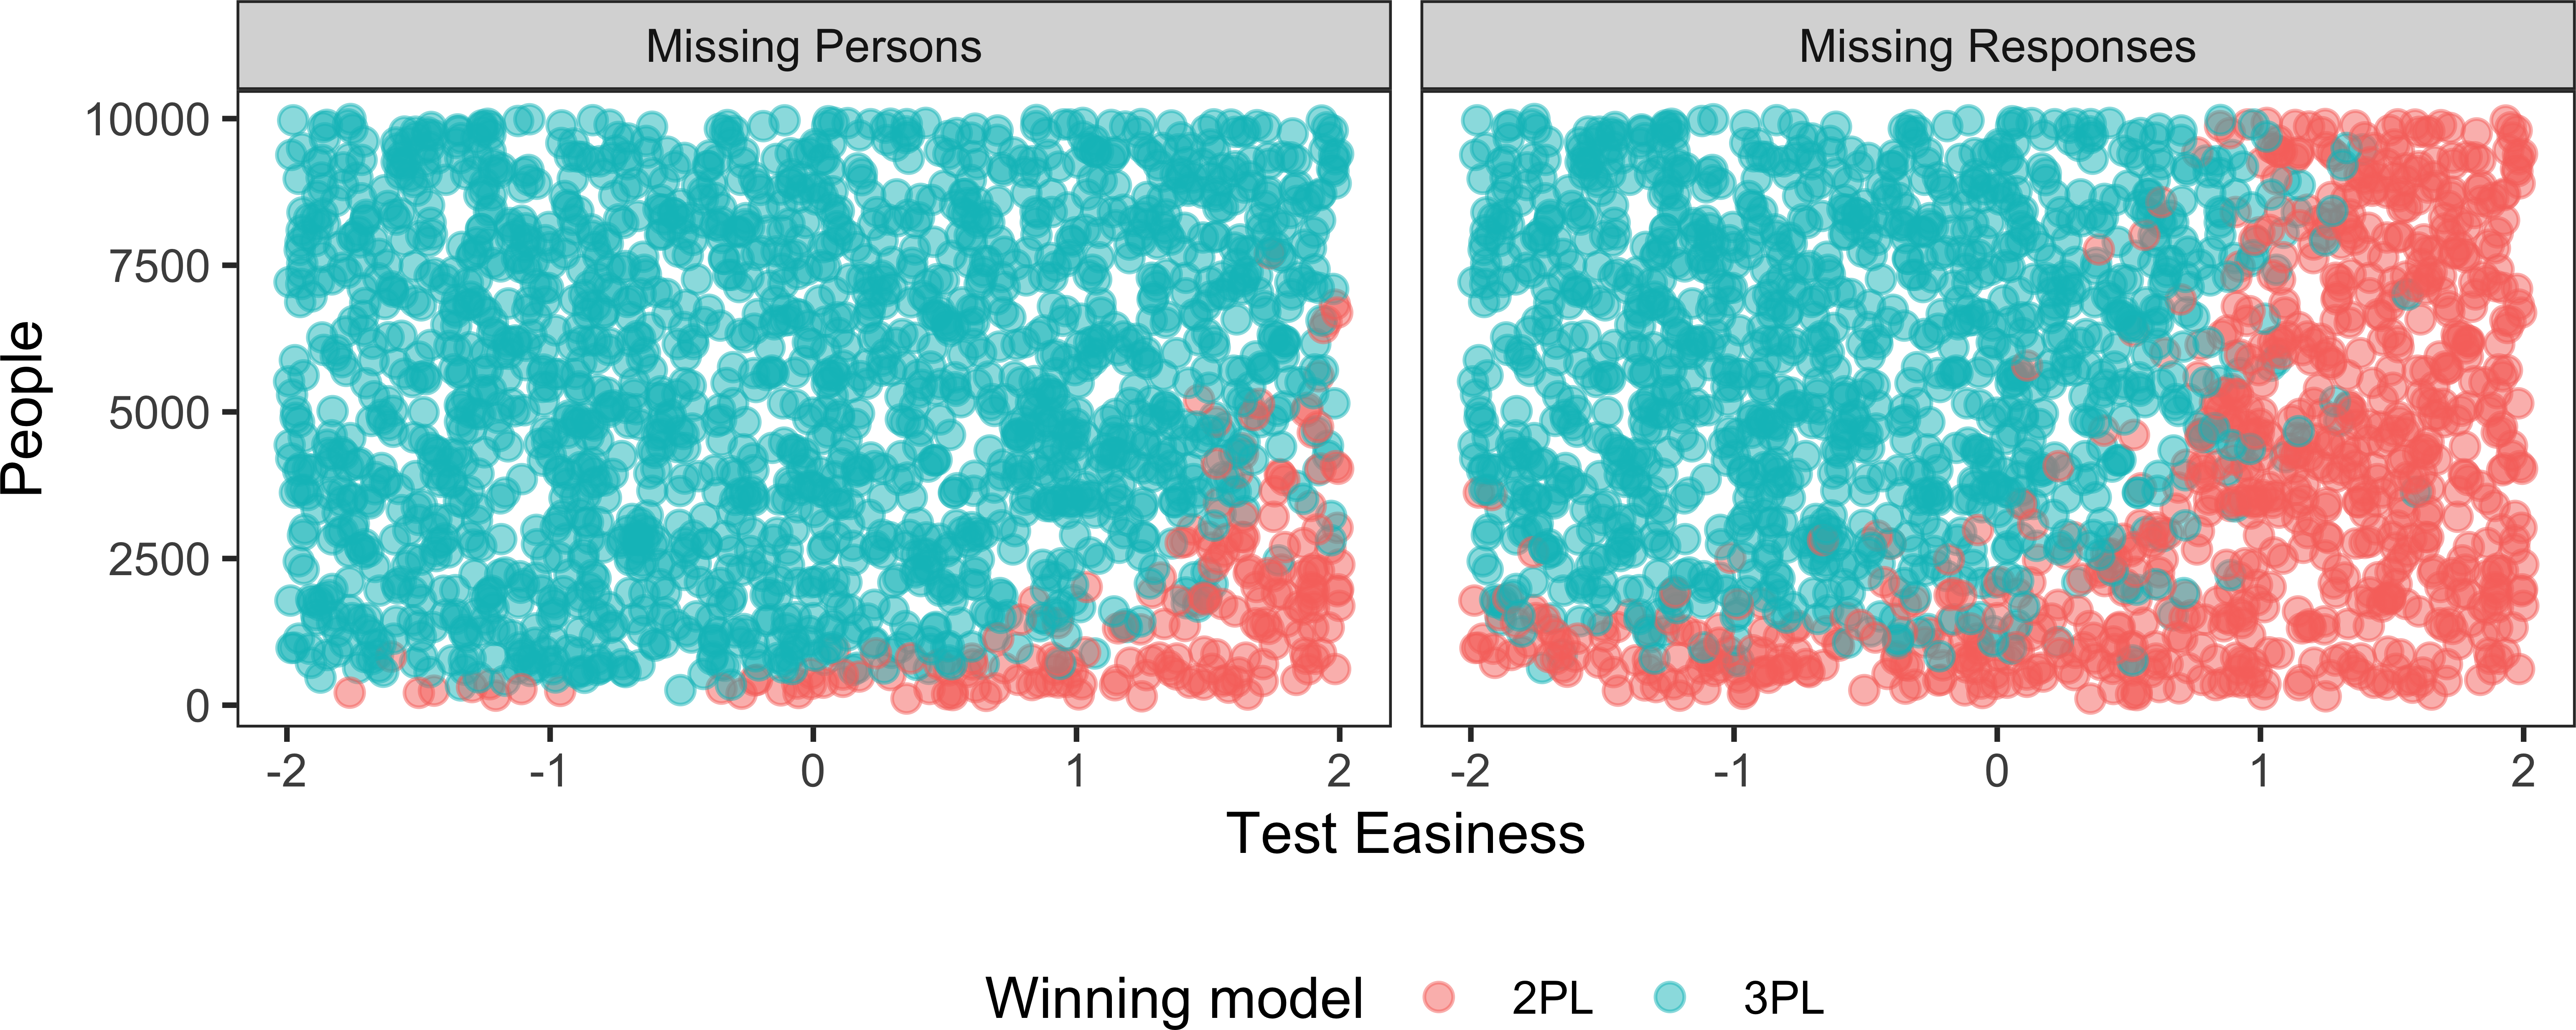
\includegraphics[width=2100px]{irt-predictive-fit-apa_files/figure-latex/results4b-1}

}

\caption{Simulation study 2 results. Each point corresponds to the prediction-maximizing model according to the predictive fit metrics, ELPL-MR and ELPL-MP, or the model selected by BIC, AIC, or LRT for one of 2000 replications. The 3PL model was most likely to offer the best fit and be selected with more persons and at lower mean ability (guessing is more prominent). For the predictive fit metrics, ELPL-MP preferred more flexible models than ELPL-MR. For the model selection methods, LRT and AIC preferred more flexible models than BIC.}\label{fig:results4b}
\end{figure}

\hypertarget{methods-for-simulation-study-3}{%
\subsection{Methods for Simulation Study 3}\label{methods-for-simulation-study-3}}

Simulation Studies 1 and 2 both used item parameters from Kang and Cohen (2007). In Simulation Study 3, we simulated item parameters with the goal of understanding how different item architectures---the distribution of easiness, discrimination, and guessing---effect which model wins according to ELPL-MR and ELPL-MP. Simulation Study 3 again exclusively used the 3PL DGM. We first created nine conditions by crossing the vector of guessing parameters \(c\) (set to 0.03, 0.10, 0.25 for all items) and the sample size (set to 1000, 5000, or 10000 persons). We conducted 1000 replications in each condition, each of which was as follows. We drew 20 item easiness parameters from a normal distribution, \(b \sim N(\mu_{\text{easy}, 1})\), and we drew the mean of that distribution from a continuous uniform distribution, \(\mu_{\theta} \sim \text{unif}(-2, 2)\). Similarly, we drew 20 item discrimination parameters from a log-normal distribution, \(a \sim \text{Lognormal}(\mu_{a}, 0.5)\), and we drew \(\mu_{a}\) from a continuous uniform distribution, \(\mu_{a} \sim \text{unif}(-0.5, 1.5)\). Note that \(\mu_{a}\) is the log of the median of the log-normal distribution so, for example, when \(\mu_{a} = -0.5\), the expected median item discrimination is \(\exp(-0.5) \approx 0.61\). As in Simulation Study 1 and 2, for each replication, we fit the 1PL, 2PL, and 3PL models determined the prediction-maximizing model according to ELPL-MR and ELPL-MP, and identified the model selected by BIC, AIC, and LRT.

\hypertarget{results-for-simulation-study-3}{%
\subsection{Results for Simulation Study 3}\label{results-for-simulation-study-3}}

Figure \ref{fig:results5b1} shows the prediction-maximizing model for each replication according to ELPL-MR and ELPL-MP. As with Simulation Study 1 and 2, the 3PL model fit best more frequently according to ELPL-MP than ELPL-MR. The role of item easiness was as expected\footnote{In Simulation Study 2, the item easiness parameters were fixed and we varied the mean of ability. In Simulation Study 3, the ability distribution was fixed and we varied the mean of the item easiness parameters. The impact is the same: What matters is the difference between ability and item easiness.} from Simulation Study 2: As \(\mu_{\text{easy}}\) decreased, the 3PL model was more likely to win. Figure \ref{fig:results5b2} shows the model selected by BIC, AIC, and LRT. Consistent with results from the previous two simulation studies, LRT selected models consistent with ELPL-MP, while BIC and AIC selected models more consistent with ELPL-MR.

As anticipated, the guessing parameter played a prominent role: The 3PL model usually won when \(c = 0.25\), with the lowest sample size \(I = 1000\) using ELPL-MR as an exception. Our original hypothesis was that \(c = 0.03\) was a nearly ignorable level of guessing and consequently that the 3PL model would not perform well. That turned out not to be the case: The 3PL model won somewhat frequently even when \(c = 0.03\). Turning to discrimination, as \(\mu_{a}\) increased (so that overall item discrimination increased), the 2PL model performed worse. This result might seem counter-intuitive, but consider the following: For items with very high discriminations (i.e., nearly Guttman (1974) items), low-ability persons have very low probabilities of correct responses under the 2PL model, whereas in fact the true probability is never below the guessing parameter. This leads to the 2PL model performing poorly for items generated with high discrimination and some guessing.

\begin{figure}

{\centering 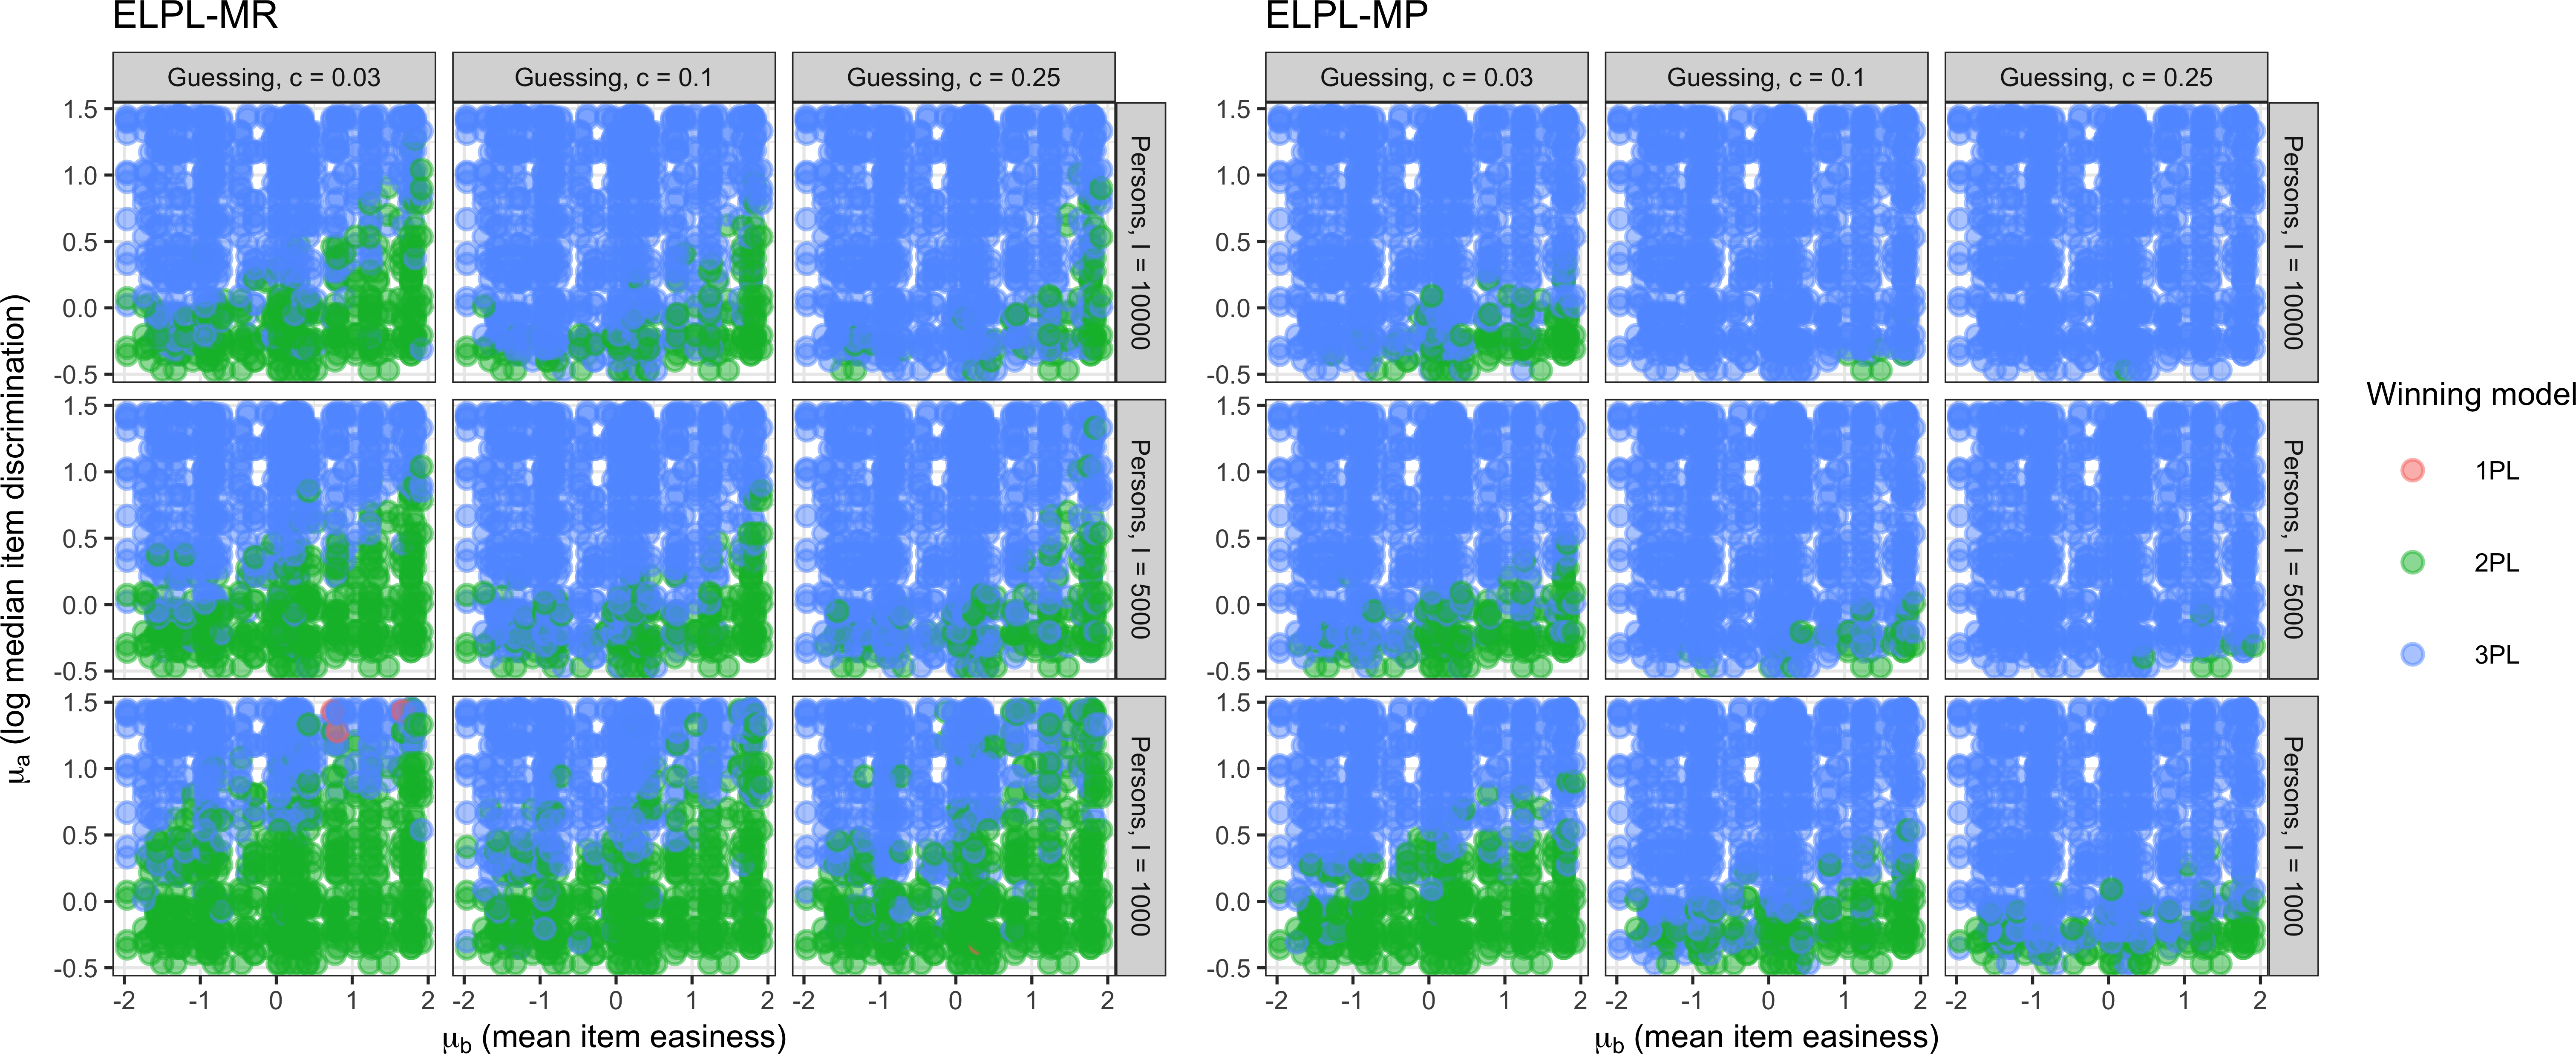
\includegraphics[width=2100px]{irt-predictive-fit-apa_files/figure-latex/results5b1-1}

}

\caption{Simulation study 3 results for the predictive fit metrics, ELPL-MR and ELPL-MP. Each point corresponds to the prediction-maximizing model from one of 1000 replications. The 3PL model was most likely to offer the best fit with greater item discrimination, more difficult items, and more persons. ELPL-MP preferred the 3PL model more often than ELPL-MR did.}\label{fig:results5b1}
\end{figure}

\begin{figure}

{\centering 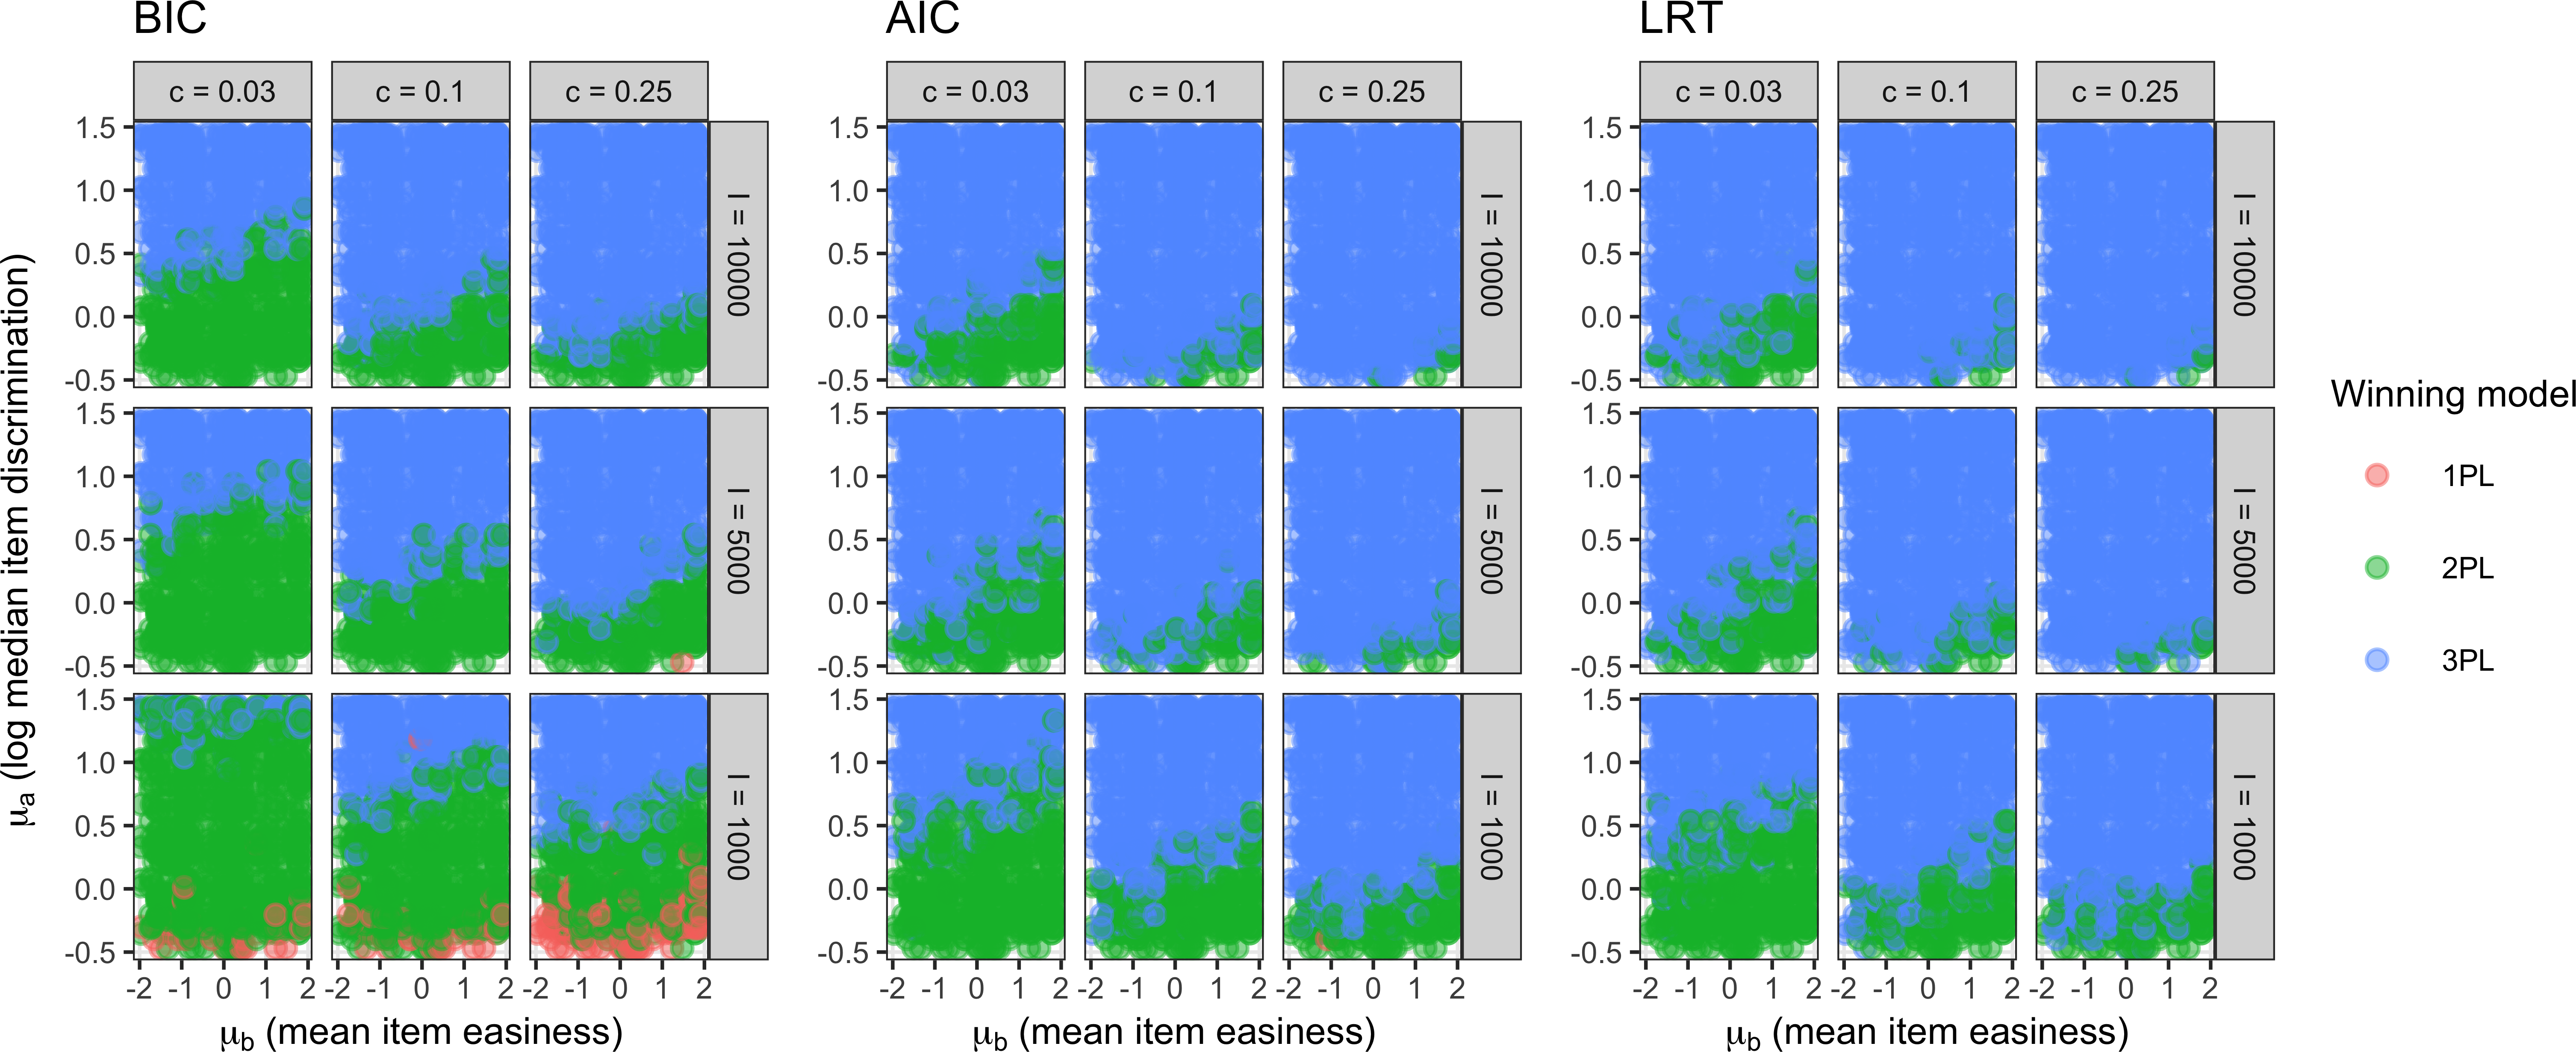
\includegraphics[width=2100px]{irt-predictive-fit-apa_files/figure-latex/results5b2-1}

}

\caption{Simulation study 3 results for the model selection methods, BIC, AIC, and LRT. Each point corresponds to the selected model from one of 1000 replications. The 3PL model was selected more often with greater item discrimination, more difficult items, and more persons. BIC selected models consistent with ELPL-MR, while AIC and LRT selected models more consistent with ELPL-MP.}\label{fig:results5b2}
\end{figure}

\hypertarget{methods-for-simulation-study-4}{%
\subsection{Methods for Simulation Study 4}\label{methods-for-simulation-study-4}}

Each of the previous simulation studies looked at models with varying item complexity (e.g., 1PL, 2PL, and 3PL) but a fixed single latent ability factor. In Simulation Study 4, we invert our focus by always using a 2PL model, but varying the number of latent ability factors. For example, the 2-factor 2PL (hereafter 2F 2PL) model is specified as
\begin{equation}
\text{Pr}(Y_{ij}) = F(a_{j1}\theta_{i1} + a_{j2} \theta_{i2} + b_j)
\end{equation}
where, for example, \(a_{j2}\) is the \(j\)th item's loading on the 2nd factor, and \(\theta_{i2}\) is the \(i\)th person's score for the 2nd factor (Reckase, 2009). Our questions are similar as in the previous simulation studies: For example, if the DGM is a 2F 2PL model, when does a 1F 2PL model make better predictions for new data from the DGM as measured by ELPL-MR and ELPL-MP?

Accordingly, Simulation Study 4 used exclusively the 2F 2PL DGM. As with the previous simulation studies, we considered only 20 items. We conducted 2000 runs, each of which was as follows. We drew item easiness parameters from the standard normal distribution, \(b \sim N(0, 1)\). We drew item discrimination parameters independently\footnote{In particular, each item's loading on each factor was independent so that the first item's loading on the first factor was independent of its loading on the second factor.} from a log-normal distribution, \(a \sim \text{Lognormal}(0, 0.5)\). We drew the number of persons from a discrete uniform distribution, \(I \sim \text{unif}\{500, 10000\}\). We drew abilities from a multidimensional normal distribution with mean vector \{{[}\}\(\mu_{\theta_1} = 0\), \(\mu_{\theta_2} = 0\)\{{]}\} and covariance matrix \(\begin{bmatrix} 1 & v \\ v & 1 \end{bmatrix}\) where \(v\) is the correlation between factors and captures the degree to which persons with a high first factor score tend to have a high second factor score. For example, if the first factor is addition, and the second factor is subtraction, then we might expect \(v\) to be high. We can think of \(v\) as essentially making dimensionality continuous: At \(v = 1\), ability is unidimensional, at \(v = 0\), ability is fully two-dimensional, and at \(v = 0.5\), ability is somewhere between one and two dimensional. We drew \(v\) from a continuous uniform distribution, \(v \sim \text{unif}(0, 1)\). We conducted 2000 such replications.

\hypertarget{results-for-simulation-study-4}{%
\subsection{Results for Simulation Study 4}\label{results-for-simulation-study-4}}

Figure \ref{fig:results6a} shows the winning model for each run according to ELPL-MP (left) and ELPL-MR (right). As before, ELPL-MR preferred more parsimonious models, with the 1F 2PL winning slightly more frequently according to ELPL-MR than ELPL-MP. We focus here on the role of the correlation between factors, \(v\). In general, as \(v\) increased, the 1F 2PL was more likely to win. As with Simulation Study 2, we can read these results in terms of minimum sample requirements for the 2F 2PL model. Under these conditions, the 2F 2PL was best according to both metrics whenever \(v < 0.5\) (at least up to our minimum sample size of \(I = 500\) persons). For greater values of \(v\), the 1F 2PL was more often best, especially for lower sample sizes and according to ELPL-MR. Lastly, it's worth noting that the 2F 2PL typically won according to both metrics for \(v\) near 0.7 and \(I\) close to 10,000 persons, which suggests that at large sample sizes it's possible for multi-factor item response models to disentangle highly correlated factors.

\begin{figure}

{\centering 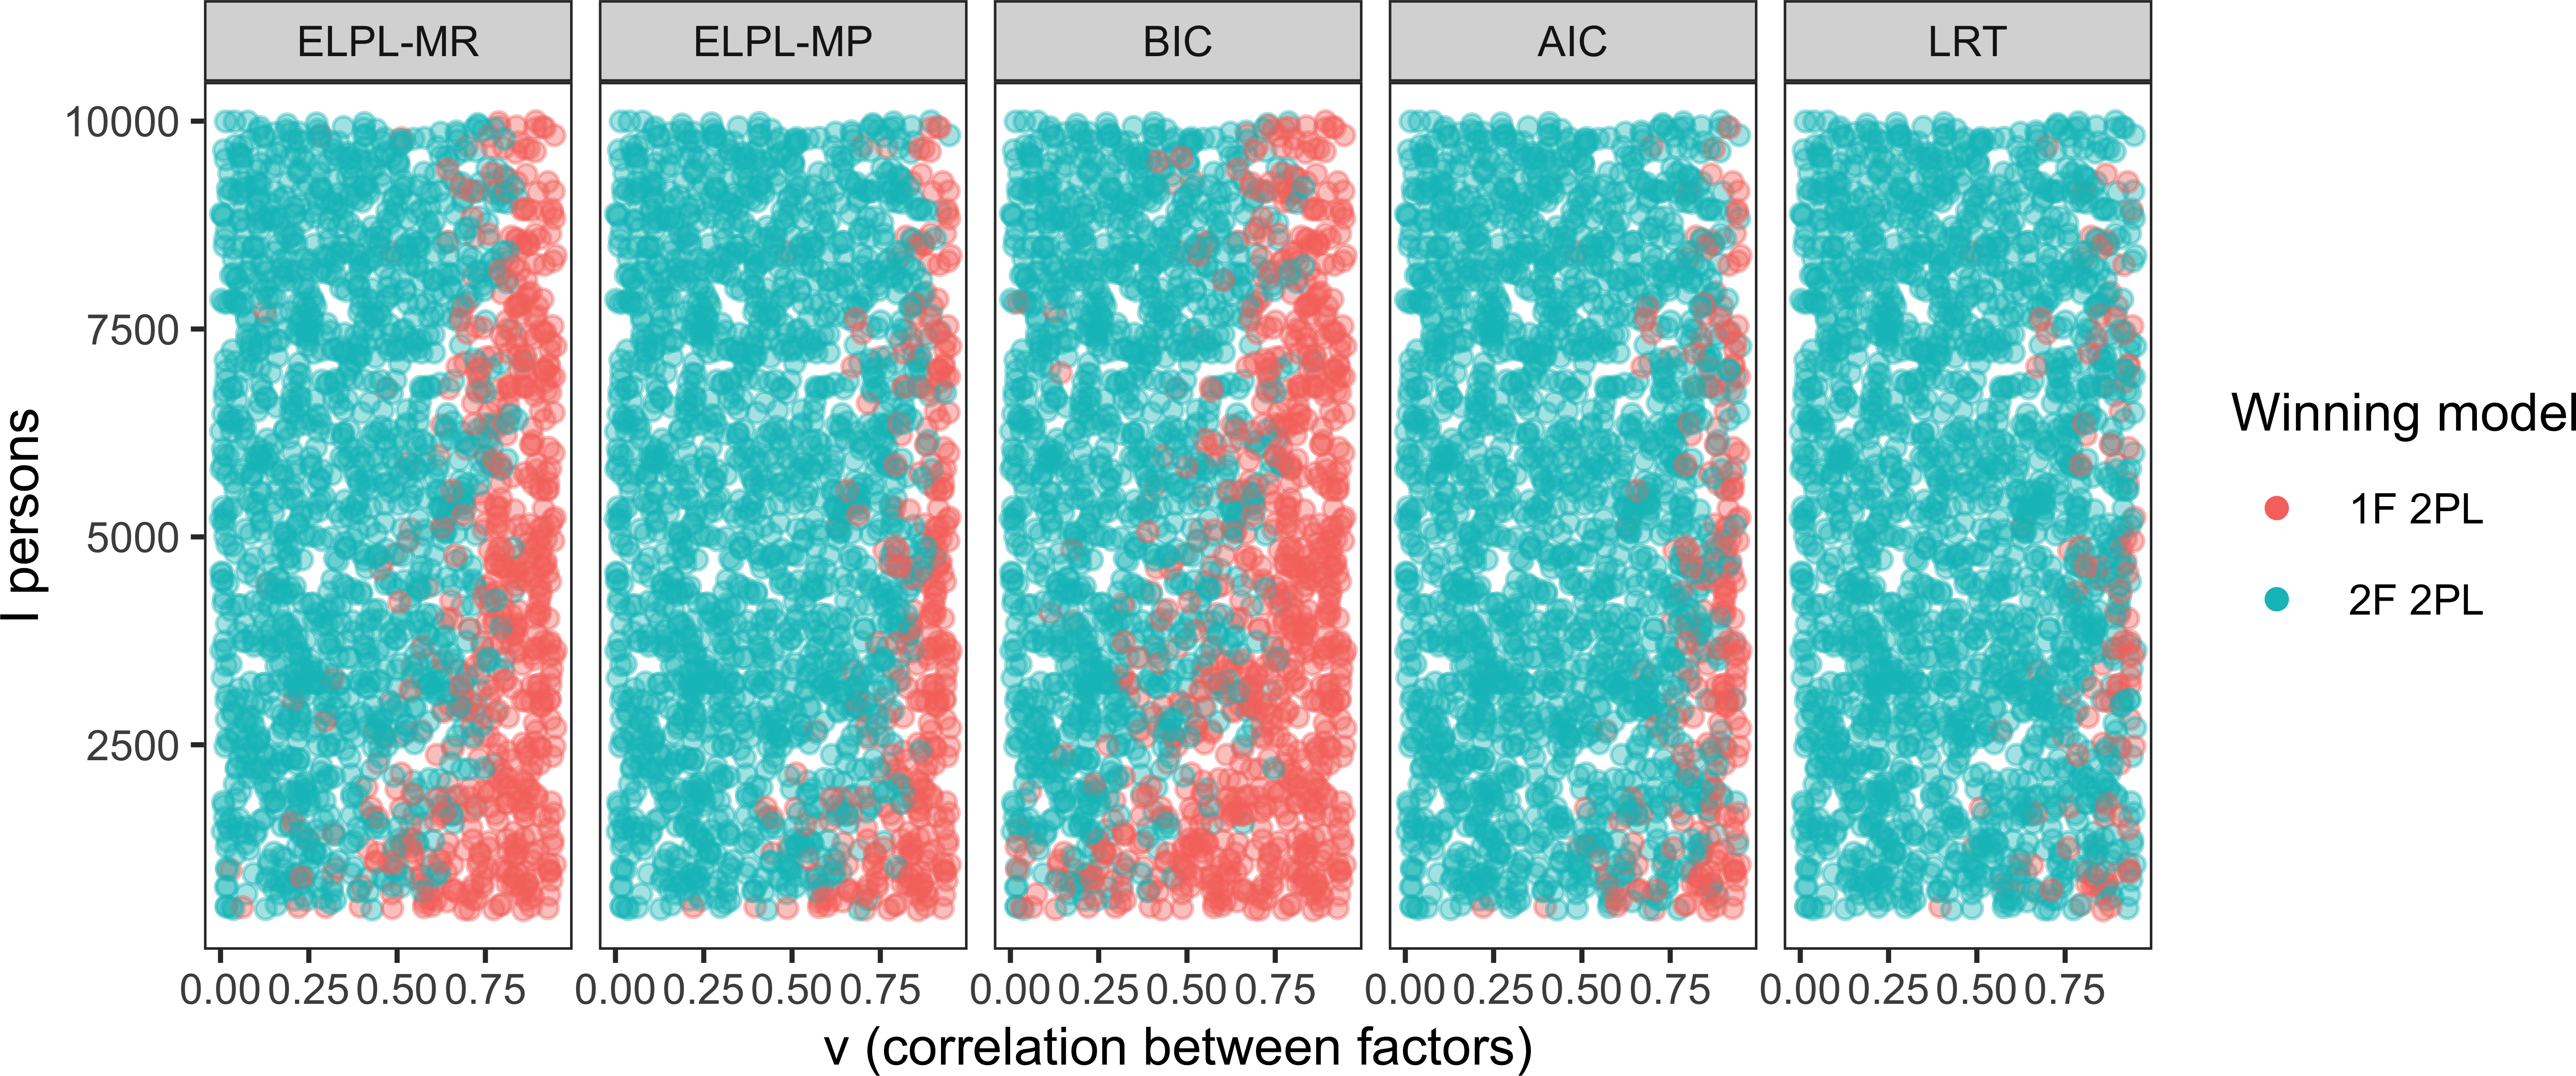
\includegraphics[width=2100px]{irt-predictive-fit-apa_files/figure-latex/results6a-1}

}

\caption{Simulation Study 4 results. Each point corresponds to the prediction-maximizing model according to the predictive fit metrics, ELPL-MR and ELPL-MP, or the model selected by BIC, AIC, or LRT for one of 2000 replications. The prediction-maximizing and selected model was more likely to be the 2F 2PL with lower correlation between factors and more persons. LRT nearly always selected the 2F 2PL model even in replications where both ELPL-MP and ELPL-MR identified the 1F 2PL model as prediction-maximizing. AIC selected models largely consistent with ELPL-MP. BIC selected models more closely aligned to ELPL-MR.}\label{fig:results6a}
\end{figure}

\hypertarget{real}{%
\section{Predictive Fit in Practice via Cross-validation}\label{real}}

In the simulation studies, we could calculate ELPL-MR and ELPL-MP because the DGM was known. In practice, when the DGM is not known, the predictive performance metrics can be estimated by hiding part of the data from the model so as to serve as out-of-sample data. This is known as cross-validation and it needs to be implemented based on which prediction task (and metric) is of interest (Bates, Hastie, \& Tibshirani, 2021). For example, Bolt and Lall (2003) implemented a cross-validation technique that corresponds to the missing person prediction task. Bergner et al. (2012) and Wu, Davis, Domingue, Piech, and Goodman (2020) cross-validated item response models in a way that corresponds to the missing responses task. We now describe how to use cross-validation to estimate each predictive fit metric in practice. We then provide a real data example of using cross-validation.

\hypertarget{cross-validated-log-likelihood-for-missing-responses-cvll-mr}{%
\subsection{Cross-validated Log Likelihood for Missing Responses (CVLL-MR)}\label{cross-validated-log-likelihood-for-missing-responses-cvll-mr}}

We randomly partition the data into folds based on the item responses (i.e., the elements of \(Y\)). We stratify randomization by person so that each person is split into ``sub-persons'' and each sub-person gets randomly assigned to a fold (DiTrapani, 2019). As a result, each fold contains approximately the same number of item responses for each person. Mathematically, following notation similar to Vehtari, Gelman, and Gabry (2017), the data is partitioned into 8 folds \(Y^{(k)}\) for \(k = 1, \dots, 8\). Each model is fit separately to each training set \(Y^{(-k)}\) using MMLE, which yields item parameter estimates \(\bm{\psi_j^{(-k)}}\). Similarly, person abilities, \(\bm{\hat\theta_i^{(-k)}}\), are estimated using EAP. The predictive (i.e.~out-of-sample or cross-validated) likelihood of \(Y^{(k)}\) is
\begin{equation}
p(Y^{(k)} | Y^{(-k)}) = \prod_{i=1}^{I} \prod_{j=1}^{J}  \hat{\text{Pr}}(y_{ij}^{(k)} | \bm{\hat\psi_j}^{(-k)}, \bm{\hat\theta_i}^{(-k)}).
\end{equation}
We then aggregate across folds to get the cross-validated log likelihood for missing responses (CVLL-MR):
\begin{equation}
\text{CVLL-MR}(\text{model}(Y)) = \sum_{k = 1}^{K} \log p(Y^{(k)} | Y^{(-k)}).
\end{equation}

\hypertarget{cross-validated-log-likelihood-for-missing-persons-cvll-mp}{%
\subsection{Cross-validated Log Likelihood for Missing Persons (CVLL-MP)}\label{cross-validated-log-likelihood-for-missing-persons-cvll-mp}}

We randomly partition the data into folds based on the persons (i.e., the rows of \(Y\)). Mathematically, the data is partitioned into 8 folds \(Y^{(k)}\) for \(k = 1, \dots, 8\). Each model is fit separately to each training set \(Y^{(-k)}\) using MMLE, which yields item parameter estimates \(\bm{\psi_j^{(-k)}}\). For each fold, we calculate predictive (i.e.~out-of-sample or cross-validated) likelihood of \(Y^{(k)}\) by integrating over \(\hat g(\bm{\theta})\):
\begin{equation}
p(Y^{(k)} | Y^{(-k)}) = \prod_{i \in i^{(k)}}^{I} \int \prod_{j=1}^{J} \hat{\text{Pr}}(y_{ij}^{(k)} | \psi_j^{(-k)}, \theta) \hat g(\bm{\theta})d\bm{\theta}.
\end{equation}
We then aggregate across folds to get the cross-validated log likelihood for missing persons (CVLL-MP):
\begin{equation}
\text{CVLL-MP}(\text{model}(Y)) = \sum_{k = 1}^{K} \log p(Y^{(k)} | Y^{(-k)}).
\end{equation}

\hypertarget{real-data-example}{%
\subsection{Real Data Example}\label{real-data-example}}

The Programme for International Student Assessment (PISA) is conducted every three years and aims to measure ``the extent to which 15-year-old students, near the end of the compulsory education, have acquired key knowledge and skills'' (Pisa, 2015). In 2015, PISA switched from using a Rasch model to a 2PL model based on research showing that the 2PL model had lower AIC and BIC (Oliveri \& Davier, 2011). To demonstrate model selection in practice, we compared a variety of models fit to a subset of the 2015 PISA data. In particular, we focused on the first 17 questions (because they have high response rates) from science booklet 25. We considered the 9800 students (regardless of country) who responded to all 17 questions. As a result, \(Y\) contained no missingness and \(9800 \cdot 17 = 166,600\) item responses. So that all items were dichotomously coded, we considered partial credit to be correct.

We compared seven models fit to this data: Rasch, 1F 2PL, 1F 3PL, 2F 2PL, 2F 3PL, 3F 2PL, and 3F 3PL. We evaluated each of these models using CVLL-MR, CVLL-MP, BIC, AIC, and LRT. For the LRT, we compared each pair of models ordered by number of parameters. We also evaluated each model using cross-validated accuracy for missing responses (CVACC-MR), which is similar to CVLL-MR but accuracy (at a 0.5 cutoff) as opposed to log likelihood is aggregated across folds. As shown in Table \ref{tab:results1}, the selected model varied by metric. Consistent with results from our simulation studies, metrics based on the MR prediction task selected models with fewer parameters than metrics based on the MP prediction task. In particular, CVLL-MR and CVACC-MR both selected the 1F 3PL. The other four metrics, which are all based on marginalized likelihood, selected either the 2F 3PL or 3F 3PL models.

This case study demonstrates that the selected model varies significantly by metric. The cross-validation metrics involve fewer assumptions, which might be good reason to prefer them to the other metrics. Even so, which cross-validation metric should be used? If the goal is to predict probabilities of item responses---for example, in developing a computer adaptive version of the PISA---then the 1F 3PL model as selected by CVLL-MR and CVACC-MR\footnote{A benefit of missing responses is that the results are easier to interpret. For CVACC-MR, the accuracy of each model are all within 0.4\% which may or may not be a small difference depending on the context. For CVLL-MR, the geometric mean of the likelihood can be reasoned about as the typical likelihood of an individual item response: For the 1F 3PL model the geometric mean is \(\exp\left(\frac{-84828}{166600}\right) = 0.601\) as opposed to \(\exp\left(\frac{-86130}{166600}\right) = 0.596\) for the 1F Rasch model.} might be used. On the other hand, if the goal is draw conclusions with regard to the item parameters, then a model with more parameters such as the 3F 3PL model as selected by CVLL-MP may be preferred. This example illustrates that there is no single best-fitting model---instead, results depend on a number of other factors including how prediction is defined.

\setlength{\tabcolsep}{2pt}
\begin{table}
\caption{Fit of seven models to a subset of the 2015 PISA data according to six metrics. Models are ordered by number of parameters. Consistent with results from the simulation studies, metrics based on the missing responses prediction task prefer models with fewer parameters (i.e., less flexible). LRT is the p-value for the model compared to the model in the previous row, which is why the first value is NA. Each of these comparisons yielded a p-value <10\textasciicircum{}-10, thus the most flexible model was selected. * indicates the winning model according to the metric.}
\centering
\begin{small}
\begin{tabular}[t]{llllllll}
\toprule
Model & Parameters & CVLL-MR & CVACC-MR & CVLL-MP & BIC & AIC & LRT\\
\midrule
1F Rasch & 18 & -86130 & 0.74454   & -89816 & 179759  & 179630 & NA\\
1F 2PL & 34 & -84921 & 0.74708     & -88844 & 177923  & 177679 & <10\textasciicircum{}-10\\
2F 2PL & 50 & -85869 & 0.74757     & -88758 & 177859  & 177499 & <10\textasciicircum{}-10\\
1F 3PL & 51 & *-84828* & *0.74782* & -88756 & 177880  & 177513 & <10\textasciicircum{}-10\\
3F 2PL & 65 & -86019 & 0.74764     & -88741 & 177915  & 177448 & <10\textasciicircum{}-10\\
2F 3PL & 67 & -85930 & 0.74734     & -88682 & *177837*  & 177355 & <10\textasciicircum{}-10\\
3F 3PL & 82 & -86049 & 0.74736     & *-88653* & 177888  & *177298* & *<10\textasciicircum{}-10*\\
\bottomrule
\end{tabular}
\end{small}
\label{tab:inpractice}
\end{table}

\hypertarget{dis}{%
\section{Discussion}\label{dis}}

How should we think about fit in the context of item response data? Previous research has frequently defined fit in terms of whether the model could have been the DGM (e.g., whether the expected contingency table from the model is similar to a contingency table of the data). We advocate for an alternative view of fit, predictive fit, based on how well a model predicts new data from the DGM. We derived two predictive fit metrics, ELPL-MR and ELPL-MP, which vary based on the meaning of out-of-sample for item responses. We derived these metrics in the theoretical case in which the DGM is a known item response model as is often the case in item response simulation studies and also provide an example of how they can be used in practice. As we describe below, we believe that these predictive fit metrics can help lay the groundwork for future advances in item response model evaluation in practice; are useful for evaluating item response models in simulation studies; and that our results offer guidance with regard to minimum sample size requirements for item response models.

We believe that predictive fit metrics can play a valuable role in laying the groundwork for future advances in item response model selection in practice. Model selection often involves comparing models with different numbers of parameters. A model with more parameters has a greater flexibility with which to fit the data-generating process but with this flexibility comes greater variance. A model with fewer parameters will have more stable estimates but with the stability comes potential bias. This is the well-known bias-variance trade off (Doroudi, 2020). Results from the simulation studies can be generalized in terms of this tradeoff. First, the prediction-maximizing model according to ELPL-MP was always more flexible than according to ELPL-MR. In other words, the model that is best for the missing persons prediction task typically has more parameters than the model that is best for the missing responses prediction task. Second, AIC, BIC, and LRT varied across simulation studies in their ability to select the model that generated the best predictions. LRT selected the most flexible models, while BIC selected the least flexible models. LRT tended to select models that were even more flexible than ELPL-MP identified as prediction-maximizing, while BIC tended to select models that were even more conservative than ELPL-MR identified as prediction-maximizing.

In the real world example with PISA data, metrics based on the missing persons prediction task (CVLL-MP, AIC, BIC, and LRT) selected more flexible models than metrics based on the missing responses prediction task (CVLL-MR and CVACC-MR), which is generally consistent with results from the simulation studies. However, BIC selected a fairly flexible model (the 2F 3PL model) which is surprising given our simulation study results that showed BIC to be very conservative. One possible reason for this discrepancy is McDonald and Mok (1995)'s warning that AIC and BIC may fail with modest sample sizes or misspecified models. A solution is to use cross-validation which directly estimates the predictive fit metrics and requires fewer assumptions (Bates, Hastie, \& Tibshirani, 2021; Fang, 2011). We briefly described cross-validation in our real-world example but more research is needed to guide IRT practitioners in using cross-validation. For example: How many folds are necessary in k-fold cross-validation? How much better do estimates of the predictive fit metrics get as more folds are used?

This work offers more direct guidance on how models should be evaluated in simulation studies. For example, Kang and Cohen (2007) fit both a 2PL and 3PL model to data from a 3PL DGM. How should they have decided whether the 2PL model or the 3PL model fit better? They assumed that because the 3PL DGM was used that the 3PL model must fit better. Based on this assumption, they, for example, warned against using a model selection method because it frequently selected the 2PL model. An alternative is to consider predictive fit by determining which model makes the best predictions for additional data from the DGM. Results from our Simulation Study 1 demonstrate that in the conditions used in Kang and Cohen (2007), the 2PL model frequently actually makes better predictions than the 3PL model, and therefore has better predictive fit. Thus, it is a feature, not a bug, for a model selection method to select the 2PL model in these conditions. Our broader point is that predictive fit metrics should be considered in these types of simulation studies, and that using them has the potential to fundamentally change the study's conclusions.

Our simulation study results also offer guidance on a question of great practical importance: minimum sample size requirements for item response models. A variety of minimum sample size recommendations have been made for the 3PL model: Feuerstahler (2019) suggest at least 5000 persons, Hulin, Lissak, and Drasgow (1982) suggest at least 1000 persons, and Thissen and Wainer (1982) suggest at least 100,000 persons. Despite these recommendations, Feuerstahler (2019) reports that ``it is not uncommon to see the 3PL'' model fit to item response data with fewer than 1000 persons (p.~12). In our view, a reasonable approach for benchmarking the minimum sample size for the 3PL model is to consider the sample size at which the 3PL model makes better predictions than the 2PL model. This is, of course, precisely what we investigate in the first three simulation studies. Our results indicate that the minimum sample size for the 3PL model depends on a variety of considerations, including how out-of-sample is defined, the ability of the persons, and the architecture of the items. For example, considering MR, greater average person ability, and greater item discrimination are all associated with the 3PL model producing relatively worse predictions, and thus greater minimum sample sizes for the 3PL model. Still, heuristics can be useful to practitioners: Simulation Study 2 results suggest a minimum sample size for the 3PL model of at least 1000 persons according to ELPL-MR and between 500 and 1000 persons according to ELPL-MP. With regard to multidimensional models, Simulation Study 4 results demonstrate that the minimum sample size requirement for the 2F 2PL model, defined by when the 2F 2PL model makes better predictions than the 1F 2PL model, depends greatly on the correlation between factors.

We close with a fundamental question: How should item response models be evaluated and compared in practice? Should information criterion such as AIC and BIC, MP cross-validation where the empirical data is split at the \emph{person level}, or MR cross-validation where the data is split at the \emph{item response level} be used? We believe that the answer likely depends on the purpose of the model. For example, the best model comparison method for selecting a model to identify poorly performing items might very well be different than that for selecting a model to rank-order persons. In the end, ELPL-MR and ELPL-MP are simply different ways of measuring the predictive performance of an item response model. High predictive performance is a desirable property for a model, but it certainly isn't the only consideration (Vehtari, Gelman, \& Gabry, 2017). Future research might work to build a framework for comparing item response models in practice that helps researchers systematically balance the many considerations when navigating the process of starting with item response data, fitting a variety of models, and then selecting one of those models for a specific purpose.

\clearpage

\hypertarget{references}{%
\section{References}\label{references}}

\begingroup
\setlength{\parindent}{-0.5in}
\setlength{\leftskip}{0.5in}

\hypertarget{refs}{}
\begin{CSLReferences}{1}{0}
\leavevmode\hypertarget{ref-akaike1974new}{}%
Akaike, H. (1974). A new look at the statistical model identification. \emph{IEEE Transactions on Automatic Control}, \emph{19}(6), 716--723.

\leavevmode\hypertarget{ref-andersen1973goodness}{}%
Andersen, E. B. (1973). A goodness of fit test for the rasch model. \emph{Psychometrika}, \emph{38}(1), 123--140.

\leavevmode\hypertarget{ref-baker2004item}{}%
Baker, F. B., \& Kim, S.-H. (2004). \emph{Item response theory: Parameter estimation techniques}. CRC Press.

\leavevmode\hypertarget{ref-bates2021cross}{}%
Bates, S., Hastie, T., \& Tibshirani, R. (2021). Cross-validation: What does it estimate and how well does it do it? \emph{arXiv Preprint arXiv:2104.00673}.

\leavevmode\hypertarget{ref-bergner2012model}{}%
Bergner, Y., Droschler, S., Kortemeyer, G., Rayyan, S., Seaton, D., \& Pritchard, D. E. (2012). Model-based collaborative filtering analysis of student response data: Machine-learning item response theory. \emph{International Educational Data Mining Society}.

\leavevmode\hypertarget{ref-birnbaum1968some}{}%
Birnbaum, A. L. (1968). Some latent trait models and their use in inferring an examinee's ability. \emph{Statistical Theories of Mental Test Scores}.

\leavevmode\hypertarget{ref-bock1983discrete}{}%
Bock. (1983). The discrete bayesian. \emph{Modern Advances in Psychometric Research}, 103--115.

\leavevmode\hypertarget{ref-bock1981marginal}{}%
Bock, \& Aitkin, M. (1981). Marginal maximum likelihood estimation of item parameters: Application of an EM algorithm. \emph{Psychometrika}, \emph{46}(4), 443--459.

\leavevmode\hypertarget{ref-bolt2003estimation}{}%
Bolt, D. M., \& Lall, V. F. (2003). Estimation of compensatory and noncompensatory multidimensional item response models using markov chain monte carlo. \emph{Applied Psychological Measurement}, \emph{27}(6), 395--414.

\leavevmode\hypertarget{ref-casabianca2015irt}{}%
Casabianca, J. M., \& Lewis, C. (2015). IRT item parameter recovery with marginal maximum likelihood estimation using loglinear smoothing models. \emph{Journal of Educational and Behavioral Statistics}, \emph{40}(6), 547--578.

\leavevmode\hypertarget{ref-chalmers2012mirt}{}%
Chalmers, R. P. (2012). Mirt: A multidimensional item response theory package for the r environment. \emph{Journal of Statistical Software}, \emph{48}(6), 1--29.

\leavevmode\hypertarget{ref-de2008random}{}%
De Boeck, P. (2008). Random item IRT models. \emph{Psychometrika}, \emph{73}(4), 533.

\leavevmode\hypertarget{ref-ditrapani2019assessing}{}%
DiTrapani, J. B. (2019). \emph{Assessing the absolute and relative performance of IRTrees using cross-validation and the RORME index} (PhD thesis). The Ohio State University.

\leavevmode\hypertarget{ref-doroudi2020bias}{}%
Doroudi, S. (2020). The bias-variance tradeoff: How data science can inform educational debates. \emph{AERA Open}, \emph{6}(4), 2332858420977208.

\leavevmode\hypertarget{ref-embretson2013item}{}%
Embretson, S. E., \& Reise, S. P. (2013). \emph{Item response theory}. Psychology Press.

\leavevmode\hypertarget{ref-fang2011asymptotic}{}%
Fang, Y. (2011). Asymptotic equivalence between cross-validations and akaike information criteria in mixed-effects models. \emph{Journal of Data Science}, \emph{9}(1), 15--21.

\leavevmode\hypertarget{ref-feuerstahlercharacterizing}{}%
Feuerstahler, L. (2019). Metric stability in item response models.

\leavevmode\hypertarget{ref-feynman1965feynman}{}%
Feynman, R. P., Leighton, R. B., \& Sands, M. (1965). The feynman lectures on physics; vol. i. \emph{American Journal of Physics}, \emph{33}(9), 750--752.

\leavevmode\hypertarget{ref-furr2017bayesian}{}%
Furr, D. C. (2017). \emph{Bayesian and frequentist cross-validation methods for explanatory item response models} (PhD thesis). UC Berkeley.

\leavevmode\hypertarget{ref-gelman2014understanding}{}%
Gelman, A., Hwang, J., \& Vehtari, A. (2014). Understanding predictive information criteria for bayesian models. \emph{Statistics and Computing}, \emph{24}(6), 997--1016.

\leavevmode\hypertarget{ref-guttman1974basis}{}%
Guttman, L. (1974). \emph{The basis for scalogram analysis}. Bobbs-Merrill, College Division.

\leavevmode\hypertarget{ref-hulin1982recovery}{}%
Hulin, C. L., Lissak, R. I., \& Drasgow, F. (1982). Recovery of two-and three-parameter logistic item characteristic curves: A monte carlo study. \emph{Applied Psychological Measurement}, \emph{6}(3), 249--260.

\leavevmode\hypertarget{ref-kang2007irt}{}%
Kang, T., \& Cohen, A. S. (2007). IRT model selection methods for dichotomous items. \emph{Applied Psychological Measurement}, \emph{31}(4), 331--358.

\leavevmode\hypertarget{ref-lord1983small}{}%
Lord, F. M. (1983). Small n justifies rasch model. In \emph{New horizons in testing} (pp. 51--61). Elsevier.

\leavevmode\hypertarget{ref-luecht2018technical}{}%
Luecht, R., \& Ackerman, T. A. (2018). A technical note on IRT simulation studies: Dealing with truth, estimates, observed data, and residuals. \emph{Educational Measurement: Issues and Practice}, \emph{37}(3), 65--76.

\leavevmode\hypertarget{ref-maydeu2013goodness}{}%
Maydeu-Olivares, Alberto. (2013). Goodness-of-fit assessment of item response theory models. \emph{Measurement: Interdisciplinary Research and Perspectives}, \emph{11}(3), 71--101.

\leavevmode\hypertarget{ref-maydeu2005limited}{}%
Maydeu-Olivares, Albert, \& Joe, H. (2005). Limited-and full-information estimation and goodness-of-fit testing in 2 n contingency tables: A unified framework. \emph{Journal of the American Statistical Association}, \emph{100}(471), 1009--1020.

\leavevmode\hypertarget{ref-mcdonald1995goodness}{}%
McDonald, R. P., \& Mok, M. M.-C. (1995). Goodness of fit in item response models. \emph{Multivariate Behavioral Research}, \emph{30}(1), 23--40.

\leavevmode\hypertarget{ref-oliveri2011investigation}{}%
Oliveri, M. E., \& Davier, M. von. (2011). Investigation of model fit and score scale comparability in international assessments. \emph{Psychological Test and Assessment Modeling}, \emph{53}(3), 315.

\leavevmode\hypertarget{ref-pisa2015pisa}{}%
Pisa, O. (2015). Pisa: Results in focus. \emph{Organisation for Economic Co-Operation and Development: OECD}.

\leavevmode\hypertarget{ref-rcore}{}%
R Core Team. (2019). \emph{R: A language and environment for statistical computing}. Vienna, Austria: R Foundation for Statistical Computing. Retrieved from \url{https://www.R-project.org/}

\leavevmode\hypertarget{ref-rasch1960probabilistic}{}%
Rasch, G. (1960). \emph{Probabilistic models for some intelligence and attainment tests.} ERIC.

\leavevmode\hypertarget{ref-reckase2009multidimensional}{}%
Reckase, M. D. (2009). Multidimensional item response theory models. In \emph{Multidimensional item response theory} (pp. 79--112). Springer.

\leavevmode\hypertarget{ref-schwarz1978estimating}{}%
Schwarz, G., \& others. (1978). Estimating the dimension of a model. \emph{Annals of Statistics}, \emph{6}(2), 461--464.

\leavevmode\hypertarget{ref-sinharay2006posterior}{}%
Sinharay, S., Johnson, M. S., \& Stern, H. S. (2006). Posterior predictive assessment of item response theory models. \emph{Applied Psychological Measurement}, \emph{30}(4), 298--321.

\leavevmode\hypertarget{ref-steiger1990structural}{}%
Steiger, J. H. (1990). Structural model evaluation and modification: An interval estimation approach. \emph{Multivariate Behavioral Research}, \emph{25}(2), 173--180.

\leavevmode\hypertarget{ref-svetina2016dimensionality}{}%
Svetina, D., \& Levy, R. (2016). Dimensionality in compensatory MIRT when complex structure exists: Evaluation of DETECT and NOHARM. \emph{The Journal of Experimental Education}, \emph{84}(2), 398--420.

\leavevmode\hypertarget{ref-thissen1982some}{}%
Thissen, D., \& Wainer, H. (1982). Some standard errors in item response theory. \emph{Psychometrika}, \emph{47}(4), 397--412.

\leavevmode\hypertarget{ref-tibshirani1996regression}{}%
Tibshirani, R. (1996). Regression shrinkage and selection via the lasso. \emph{Journal of the Royal Statistical Society: Series B (Methodological)}, \emph{58}(1), 267--288.

\leavevmode\hypertarget{ref-vehtari2017practical}{}%
Vehtari, A., Gelman, A., \& Gabry, J. (2017). Practical bayesian model evaluation using leave-one-out cross-validation and WAIC. \emph{Statistics and Computing}, \emph{27}(5), 1413--1432.

\leavevmode\hypertarget{ref-warm1989weighted}{}%
Warm, T. A. (1989). Weighted likelihood estimation of ability in item response theory. \emph{Psychometrika}, \emph{54}(3), 427--450.

\leavevmode\hypertarget{ref-watts2018explanation}{}%
Watts, D. J., Beck, E. D., Bienenstock, E. J., Bowers, J., Frank, A., Grubesic, A., \ldots{} Salganik, M. (2018). Explanation, prediction, and causality: Three sides of the same coin?

\leavevmode\hypertarget{ref-tidy}{}%
Wickham, H. (2017). \emph{Tidyverse: Easily install and load the 'tidyverse'}. Retrieved from \url{https://CRAN.R-project.org/package=tidyverse}

\leavevmode\hypertarget{ref-wu2020variational}{}%
Wu, M., Davis, R. L., Domingue, B. W., Piech, C., \& Goodman, N. (2020). Variational item response theory: Fast, accurate, and expressive. \emph{arXiv Preprint arXiv:2002.00276}.

\leavevmode\hypertarget{ref-yarkoni2017choosing}{}%
Yarkoni, T., \& Westfall, J. (2017). Choosing prediction over explanation in psychology: Lessons from machine learning. \emph{Perspectives on Psychological Science}, \emph{12}(6), 1100--1122.

\end{CSLReferences}

\endgroup


\end{document}
